\chapter{Propagating the Epistemic Uncertainty of the Cost Volume to the DSM}\label{chap:epistemic_uncertainty}
\todoroman{Citer la publication d'origine pour les figure (license IEEE ``Copyright 2024 IEEE. Published in the 2024 IEEE International Geoscience and Remote Sensing Symposium (IGARSS 2024), scheduled for 7 - 12 July, 2024 in Athens, Greece. Personal use of this material is permitted. However, permission to reprint/republish this material for advertising or promotional purposes or for creating new collective works for resale or redistribution to servers or lists, or to reuse any copyrighted component of this work in other works, must be obtained from the IEEE. Contact: Manager, Copyrights and Permissions / IEEE Service Center / 445 Hoes Lane / P.O. Box 1331 / Piscataway, NJ 08855-1331, USA. Telephone: + Intl. 908-562-3966.'')}

The previous chapter detailed the propagation of  uncertainty in a stereo matching problem, using the $\SAD$ function to compute the cost volume. However, real cases of stereo matching usually do not use such simple cost functions, but rather more complex ones. In particular, the CARS pipeline that will process the \acrshort{co3d} data will use the CENSUS and MC-CNN cost functions  \cite{zabih_non-parametric_1994,zbontar_stereo_2016} to compute the cost volume, followed by a \acrshort{sgm} regularization. Those methods produce far better results and are thus favored for stereo pipelines. Unfortunately, we are not able to propagate the uncertainty to those cost functions and regularization as we did in the previous chapter as it would be too complex and computationally heavy. The same observation can be made for any deep leaning method \cite{laga_survey_2022} as the data is processed through many consecutive layers. Furthermore, the previous chapter was restricted to the propagation of the uncertainty from input images to the cost volume, but did not attempt to quantify the uncertainty of the stereo matching process itself, \ie the algorithm ability to correctly\commanue{properly? c'est pour éviter la répétition avec correct, à moins que ce soit voulu} identify the correct disparity. A bad performing stereo matching algorithm can produce errors of great magnitude regardless of the uncertainty on input images, while more advanced algorithm may even present good performance despite noised input images. Using the semantics of this thesis, we will refer to the uncertainty of the stereo algorithm itself as its epistemic uncertainty. Indeed, it does not result form any aleatoric process, but rather a lack of knowledge on how to correctly and automatically identify the correct disparity\commanue{pareil tu as une répétition entre correctly et correct dans la phrase}.

This aforementioned epistemic uncertainty\commanue{alors moi perso je mettrais This aforementioned epistemic uncertainty modeling in stereo matching mais c'est pas une obligation} has been the subject of many works in the literature \cite{hu_quantitative_2012,  poggi_confidence_2021,wang_uncertainty_2022}, designed for so-called ``classical methods'' using cost volumes obtained from cost functions, or for learning-based methods. This uncertainty is quantified using ``confidence measures'', associating a value between $0$ and $1$ to each predicted disparity, $0$ meaning that the prediction should be questioned,  and $1$ meaning that the prediction is most certainly correct. We refer to \Cref{sec:uncertainty_pandora} for more details on confidence measures in stereo matching pipelines. In this chapter, we will study how possibility distributions are able to model the epistemic uncertainty associated with a cost volume, and then deduce disparity confidence intervals from the possibility distribution. This approach is complementary to classical confidence estimations as it is not meant to indicate whether or not we trust a prediction but rather to provide information on \textit{where} the correct disparity should be. We then propagate those disparity confidence intervals in the rest of the stereo pipeline to obtain height confidence intervals, and evaluate their performances\commanue{Est-ce que dans l'intro de ce chapitre il ne faudrait pas aussi que tu rappelles que les utilisateurs veulent un intervalle à 90\% et donc blabla comme tu es gentil, tu vas chercher à répondre à ce besoin et donc construction à fournir un intervalle de disparité à 90\%}.

\todoroman{Vérifier que dans le chapitre 1 j'insiste bien sur ce que c'est une cost curve}
\section{Producing Confidence Intervals}
\subsection{Possibility Distributions as Uncertain Models for Cost Curves}
In this section, we will detail how possibility distributions can be used to model the epistemic uncertainty associated with cost curves. We first present a quick reminder of concepts and notations regarding cost volumes presented in \Cref{sec:stereo_matching}, as we will base our model on them. Cost volume based approaches, considered here, compare every pixel from the left image $I_L$ to pixels from the same row in the right image $I_R$, in a given disparity range. The comparison is done using a cost function $f$, measuring the dissimilarity between two windows centered around pixel $p$ and $q$. All evaluations using this cost function are stored in a cost volume $C_V$:
\begin{align}
	C_V(row, ~col, ~d) = f(I_L(row, ~col), I_R(row, ~col+d))
\end{align}
where $d$ is the considered disparity. In this chapter, we consider that the cost volume then\commanue{je mettrais pas le then} undergoes a \acrshort{sgm} regularization step, which modifies the cost values\commanue{its values} to take into account more global information. Based on the observation that the disparity map is usually piece-wise regular in a scene, \acrshort{sgm} regularization has been designed to increase the cost of disparities for which no consensus exist among neighbouring pixels. This way, only disparities that seem plausible and relatively regular compared to neighbouring disparities are favored in the cost volume.

For every pixel $(row, ~col)$ from the left image, we refer to its cost curve as the cost volume at coordinates $(row,~col)$ for every considered disparity $d$, \ie the cost volume for which we fixed the first two variables. Cost curves are of much importance as we estimate the disparity of a pixel solely based on its cost curve. Indeed, we define the predicted disparity $\tilde{d}$ of a pixel $(row, ~col)$ as:
\begin{align}
	\tilde{d} = \argmin_d C_V(row, ~col, ~d)
\end{align} 
\Cref{fig:tuto_dense_matching} presents a cost curve and its true disparity. We can see that the true disparity can be correctly estimated by looking at the minimum of the cost curve.

\begin{figure}
    \centering
    \begin{subfigure}[t]{0.073\linewidth}
        \centering
        
\includegraphics[width=\linewidth]{Images/Chap_5/tuto_left_patch.png}
        \caption{}
        \label{fig:tuto_a}
    \end{subfigure}
    \hfill\begin{subfigure}[t]{\linewidth}
        \flushright
        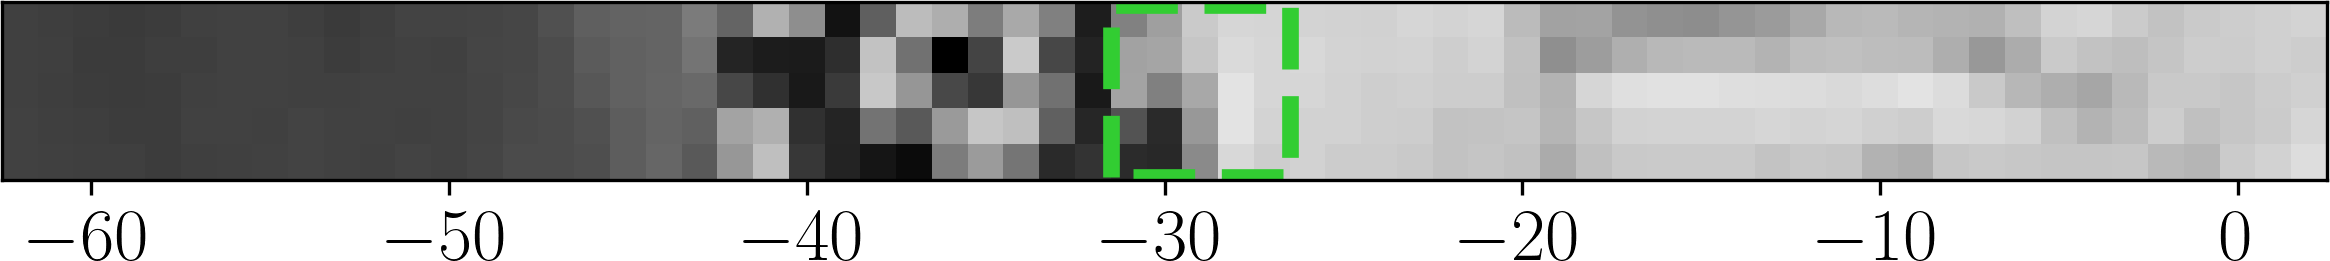
\includegraphics[width=0.927\linewidth]{Images/Chap_5/tuto_right_patch.png}
        \caption{}
        \label{fig:tuto_b}
    \end{subfigure}
    \begin{subfigure}[t]{\linewidth}
        \centering
        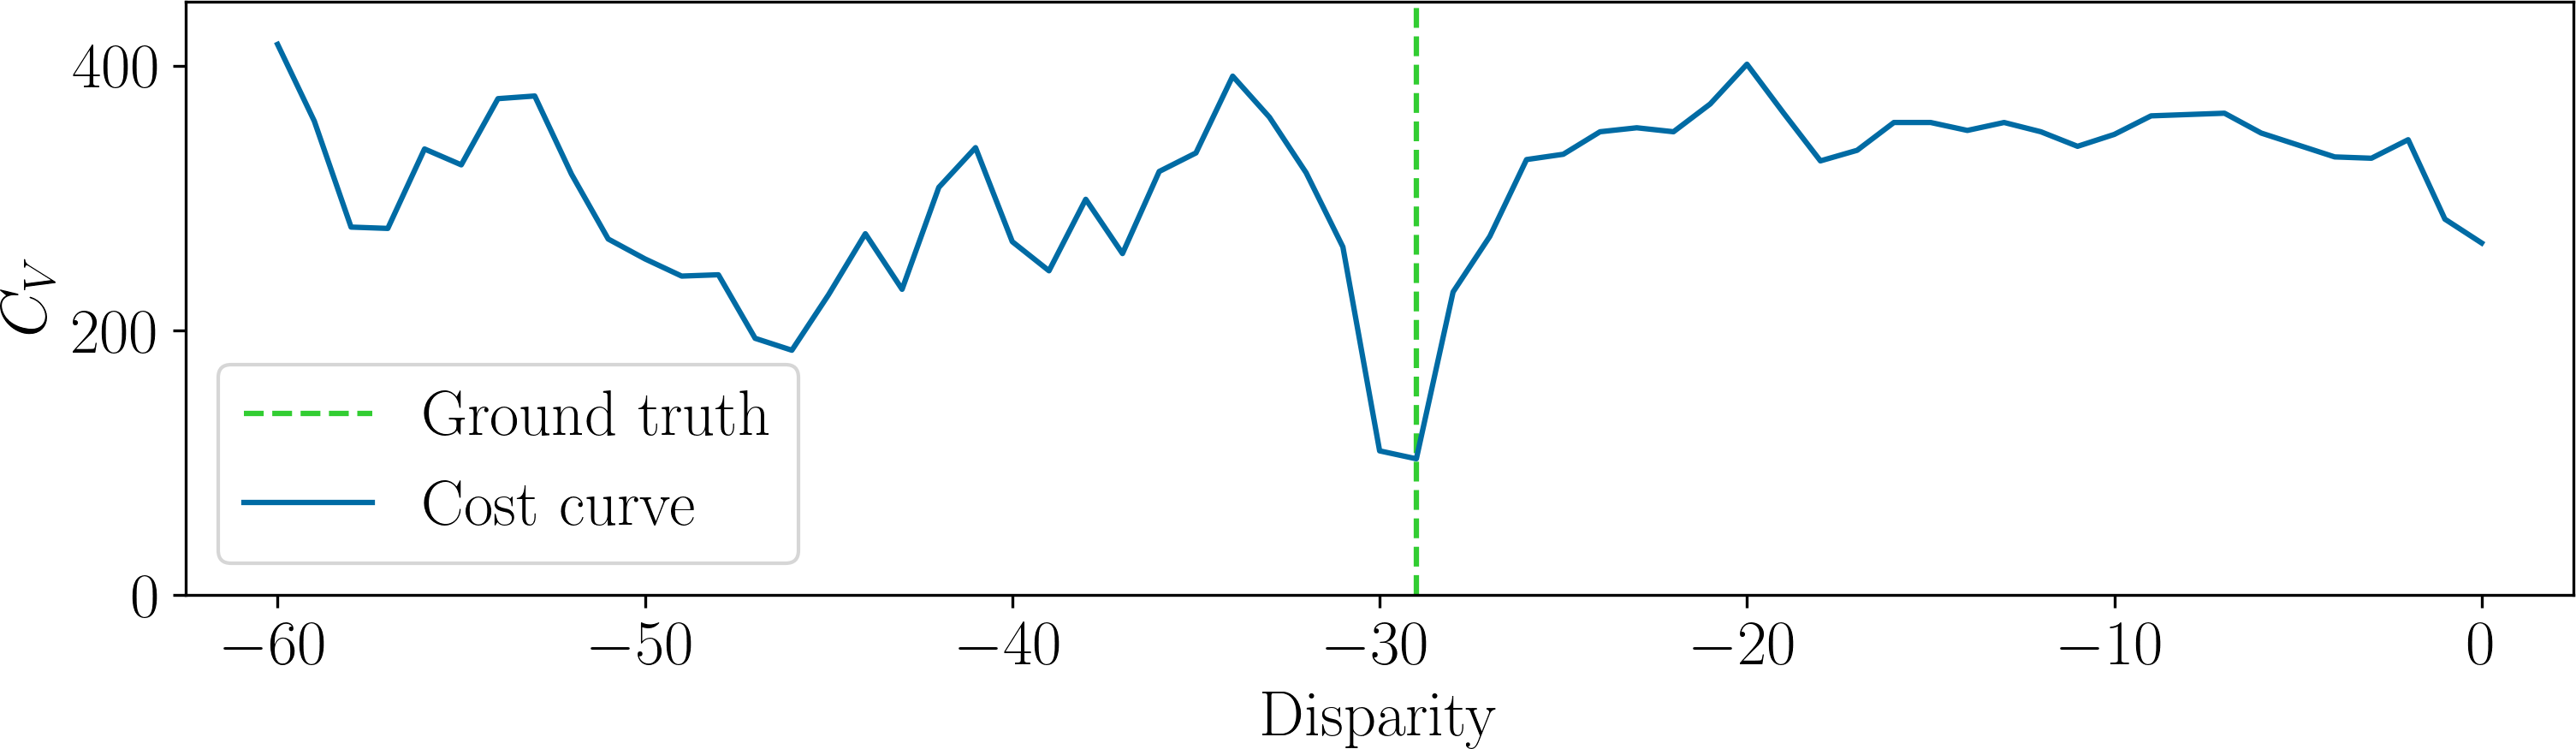
\includegraphics[width=\linewidth]{Images/Chap_5/tuto_cost_curve.png}
        \caption{Cost curve}
        \label{fig:tuto_c}
    \end{subfigure}
    \caption{Cost curve (\Cref{fig:tuto_c}) obtained from comparing a patch from the left image (\Cref{fig:tuto_a}) to patches from the right image (\Cref{fig:tuto_b}). The matching patch and its corresponding true disparity are indicated using dashed green lines.}
    \label{fig:tuto_dense_matching}
\end{figure}

In the following, we propose to consider possibility distributions to model the uncertainty associated with the choice of the predicted disparity from a cost curve. The values taken by possibility distributions will be based on the available information \ie the values of the cost volume. Before getting into details, let us justify this model. Possibility distributions are relatively simple model to use in comparison with imprecise probabilities or belief functions for instance, as we only need to specify a constraint on the atoms, and not on every event. As such, they have been used to model the uncertainty associated with an expert's opinion in applications such as groundwater contamination for instance in \cite{bardossy_l-_1995} and \cite{baudrit_joint_2007}. Since cost curves result in both:
\begin{itemize}
	\item dissimilarity measures between patches 
	\item a semi-global fusion of the information contained in the cost volume due to \acrshort{sgm} regularization
\end{itemize}it does not seem far-stretched to consider them equivalent to an expert stating his opinion on how likely two pixels should be matched. For this reason, possibility distributions seem appropriate to model the epistemic uncertainty of the cost volume.

In order to use possibility distributions, we first need to transform the available information, in our case the values contained in the cost curves, into degrees of possibility. \Cref{eq:possibility}\commanue{Plutôt que de faire référence à une équation située 100 pages avant, tu pourrais juste dire The definition of possibility distribution ou un truc équivalent} imposes that the values must lie between $0$ and $1$, and that the value $1$ must be attained at least once. We therefore propose to normalize each cost curve so that its minimal dissimilarity value equals a possibility degree of $1$, and that greater dissimilarity values are closer to $0$ in possibility. However, simply normalizing the values of each cost curve between $0$ and $1$ would artificially stretch the cost curve as seen in \Cref{fig:cost_curves_b}. It is especially blatant in the case for the orange dashed curve from \Cref{fig:cost_curves_a} as the range of its values is quite narrow compared to the blue curve, but they are both stretched to $[0,~1]$ in \Cref{fig:cost_curves_b}. In order to avoid this effect, we instead normalize every cost curve using the global minimum and global maximum of the cost volume, as:
\begin{align}
	C_V^{norm}(row, ~col, ~d) = \frac{C_V(row, ~col, ~d) - \max_{r,c,\delta}C_V(r,~c,~\delta)}{\min_{r,c,\delta}C_V(r,~c,~\delta) - \max_{r,c,\delta}C_V(r,~c,~\delta)}\label{eq:normalized_cost_curve}
\end{align}
Minima of the cost curve become maxima with this normalization. One problem remains, it is that unless the global maximum of the cost volume is attained in a cost curve, the normalized cost curve will never reach $1$. Therefore, it will not be a possibility distribution. This problem can be observed in \Cref{fig:cost_curves_c}. We thus add a constant to the normalized cost curve to obtain a possibility distribution $\pi_{row,~col}(d)$:
\begin{align}
	\pi_{row,~col}(d) = C_V^{norm}(row, ~col, ~d) + 1 - \max_\delta C_V^{norm}(row, ~col, ~\delta)\label{eq:possibility_cost_curve}
\end{align}
\Cref{fig:cost_curves_d} displays the possibility distributions obtained from the cost curves of \Cref{fig:cost_curves_a}.

\begin{figure}
    \centering
    \begin{subfigure}[t]{0.47\linewidth}
        \centering
        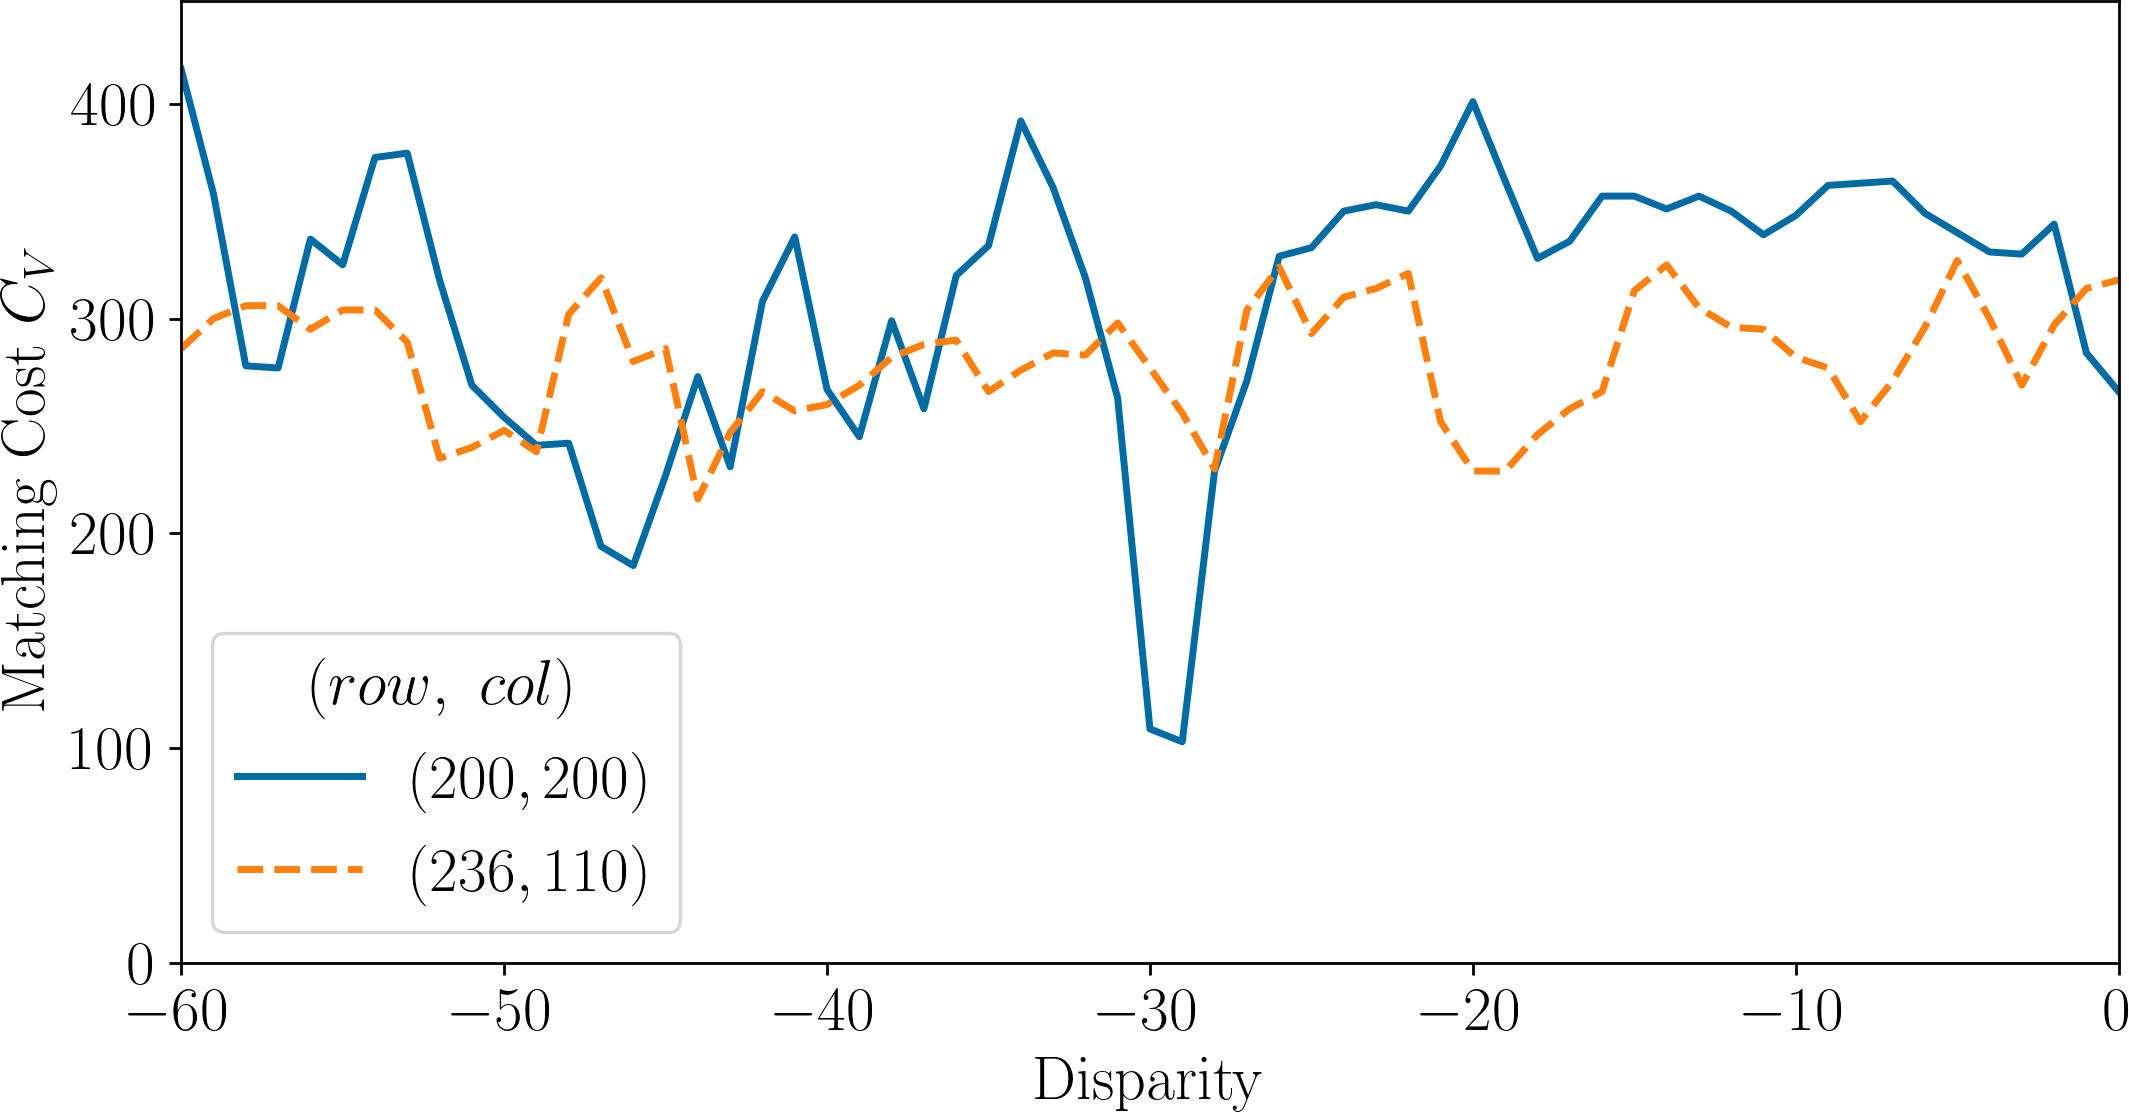
\includegraphics[width=\linewidth]{Images/Chap_5/cost_curve_not_normalized.png}
        \caption{Two cost curves}
        \label{fig:cost_curves_a}
    \end{subfigure}\hfill
    \begin{subfigure}[t]{0.47\linewidth}
        \centering
        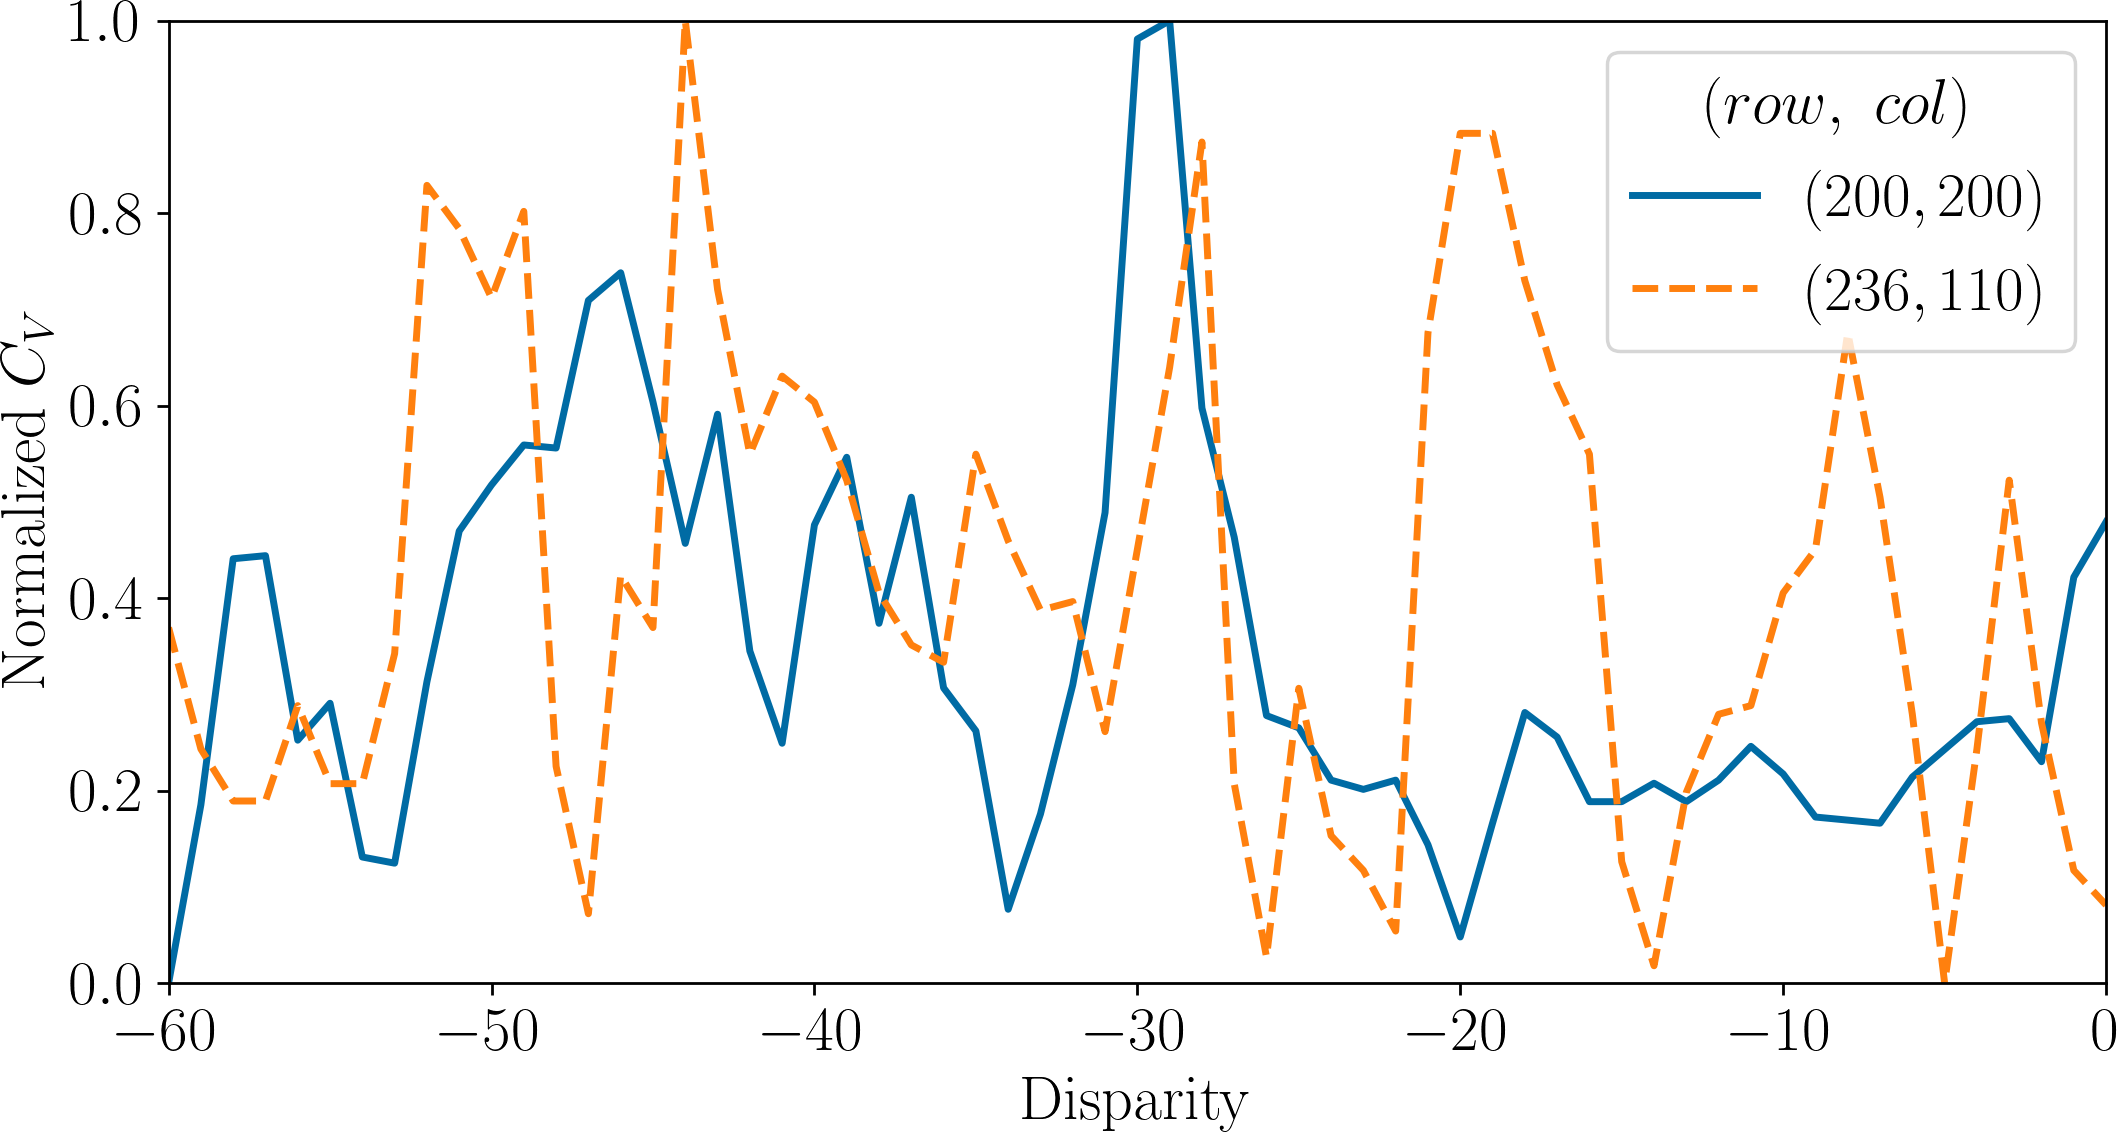
\includegraphics[width=\linewidth]{Images/Chap_5/cost_curve_bad_normalized.png}
        \caption{Normalized cost curves with local extrema}
        \label{fig:cost_curves_b}
    \end{subfigure}
    \begin{subfigure}[t]{0.47\linewidth}
        \centering
        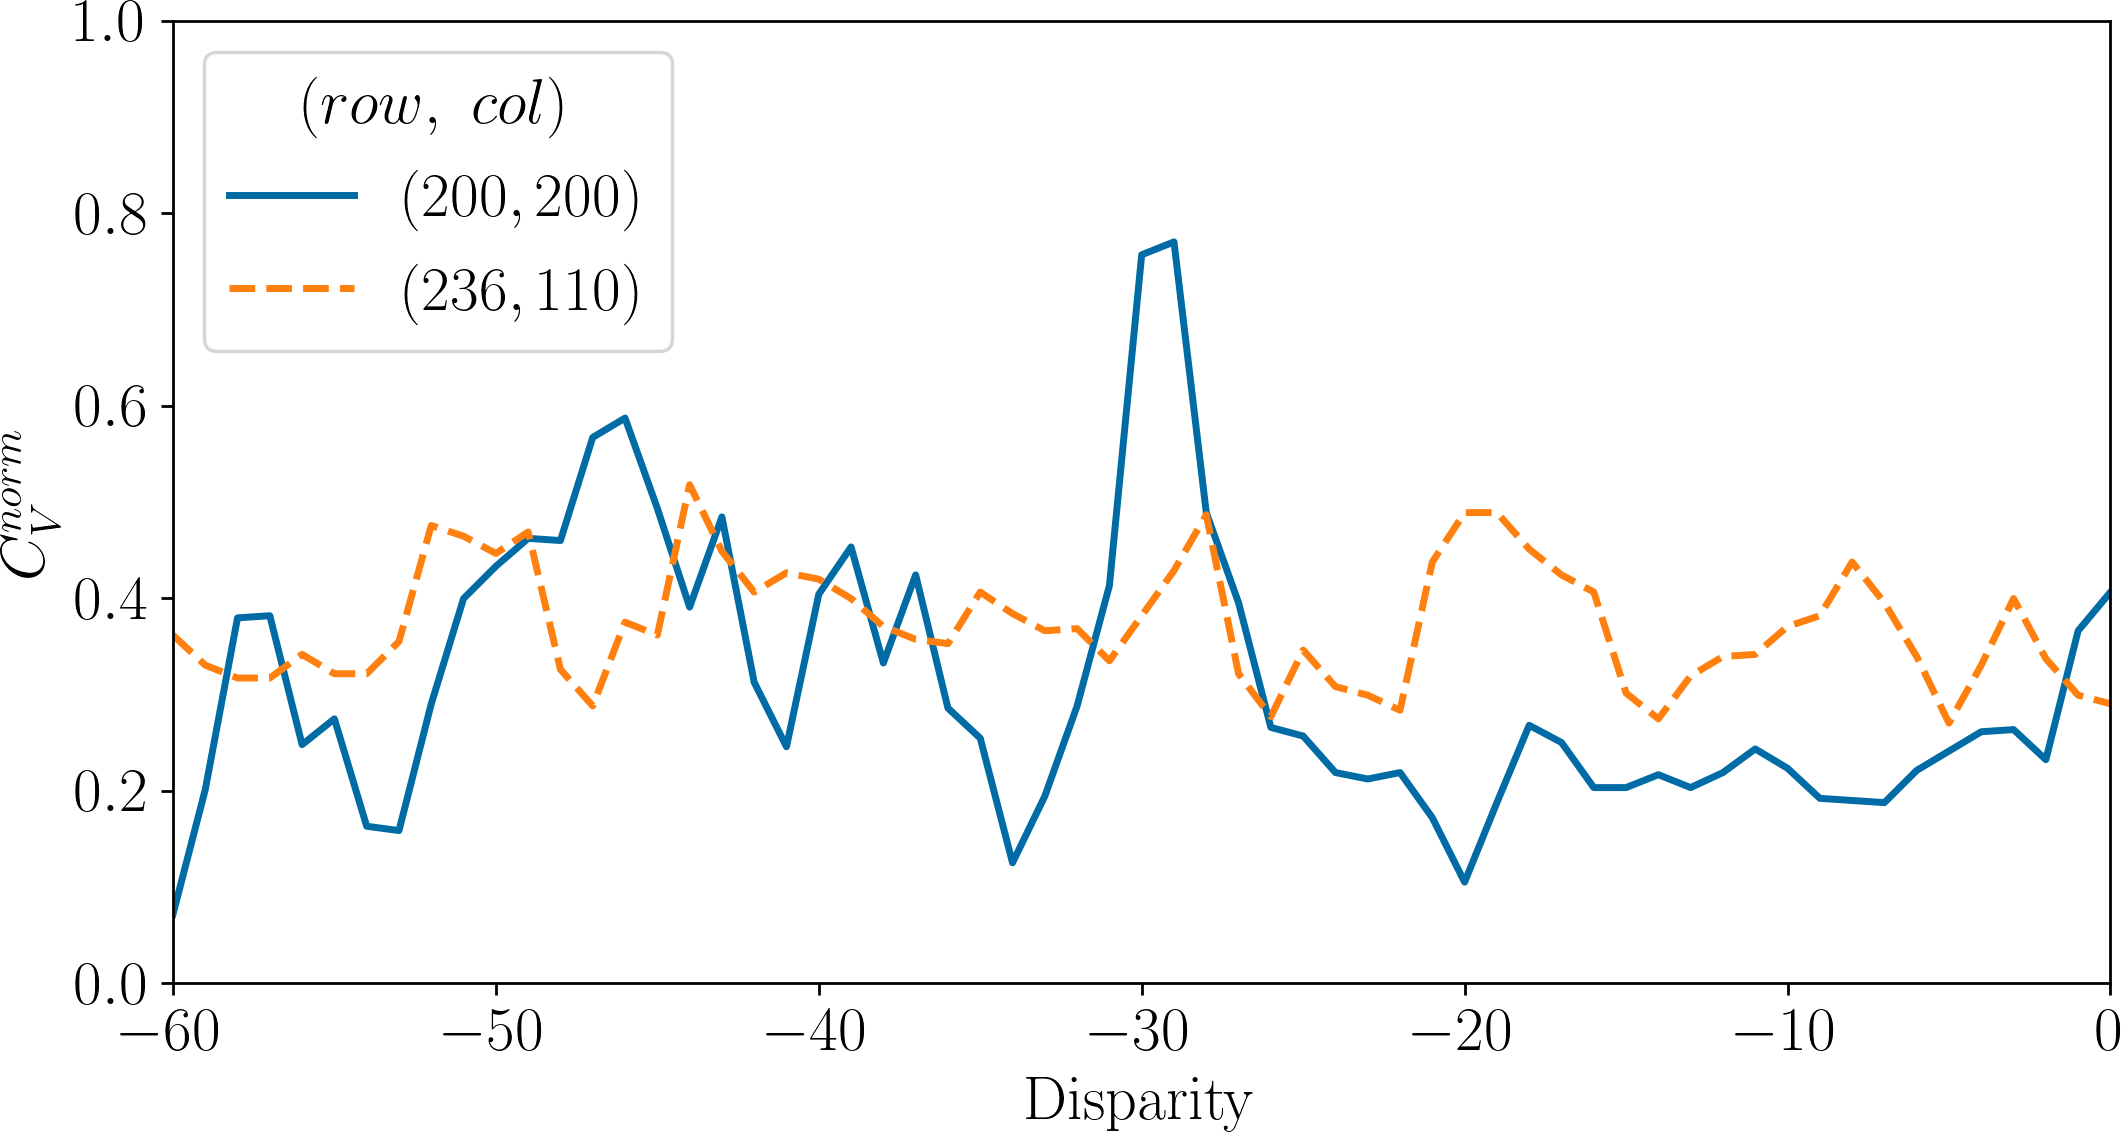
\includegraphics[width=\linewidth]{Images/Chap_5/cost_curve_normalized.png}
        \caption{Normalized cost curves $C_V^{norm}$ with global extrema}
        \label{fig:cost_curves_c}
    \end{subfigure}\hfill
    \begin{subfigure}[t]{0.47\linewidth}
        \centering
        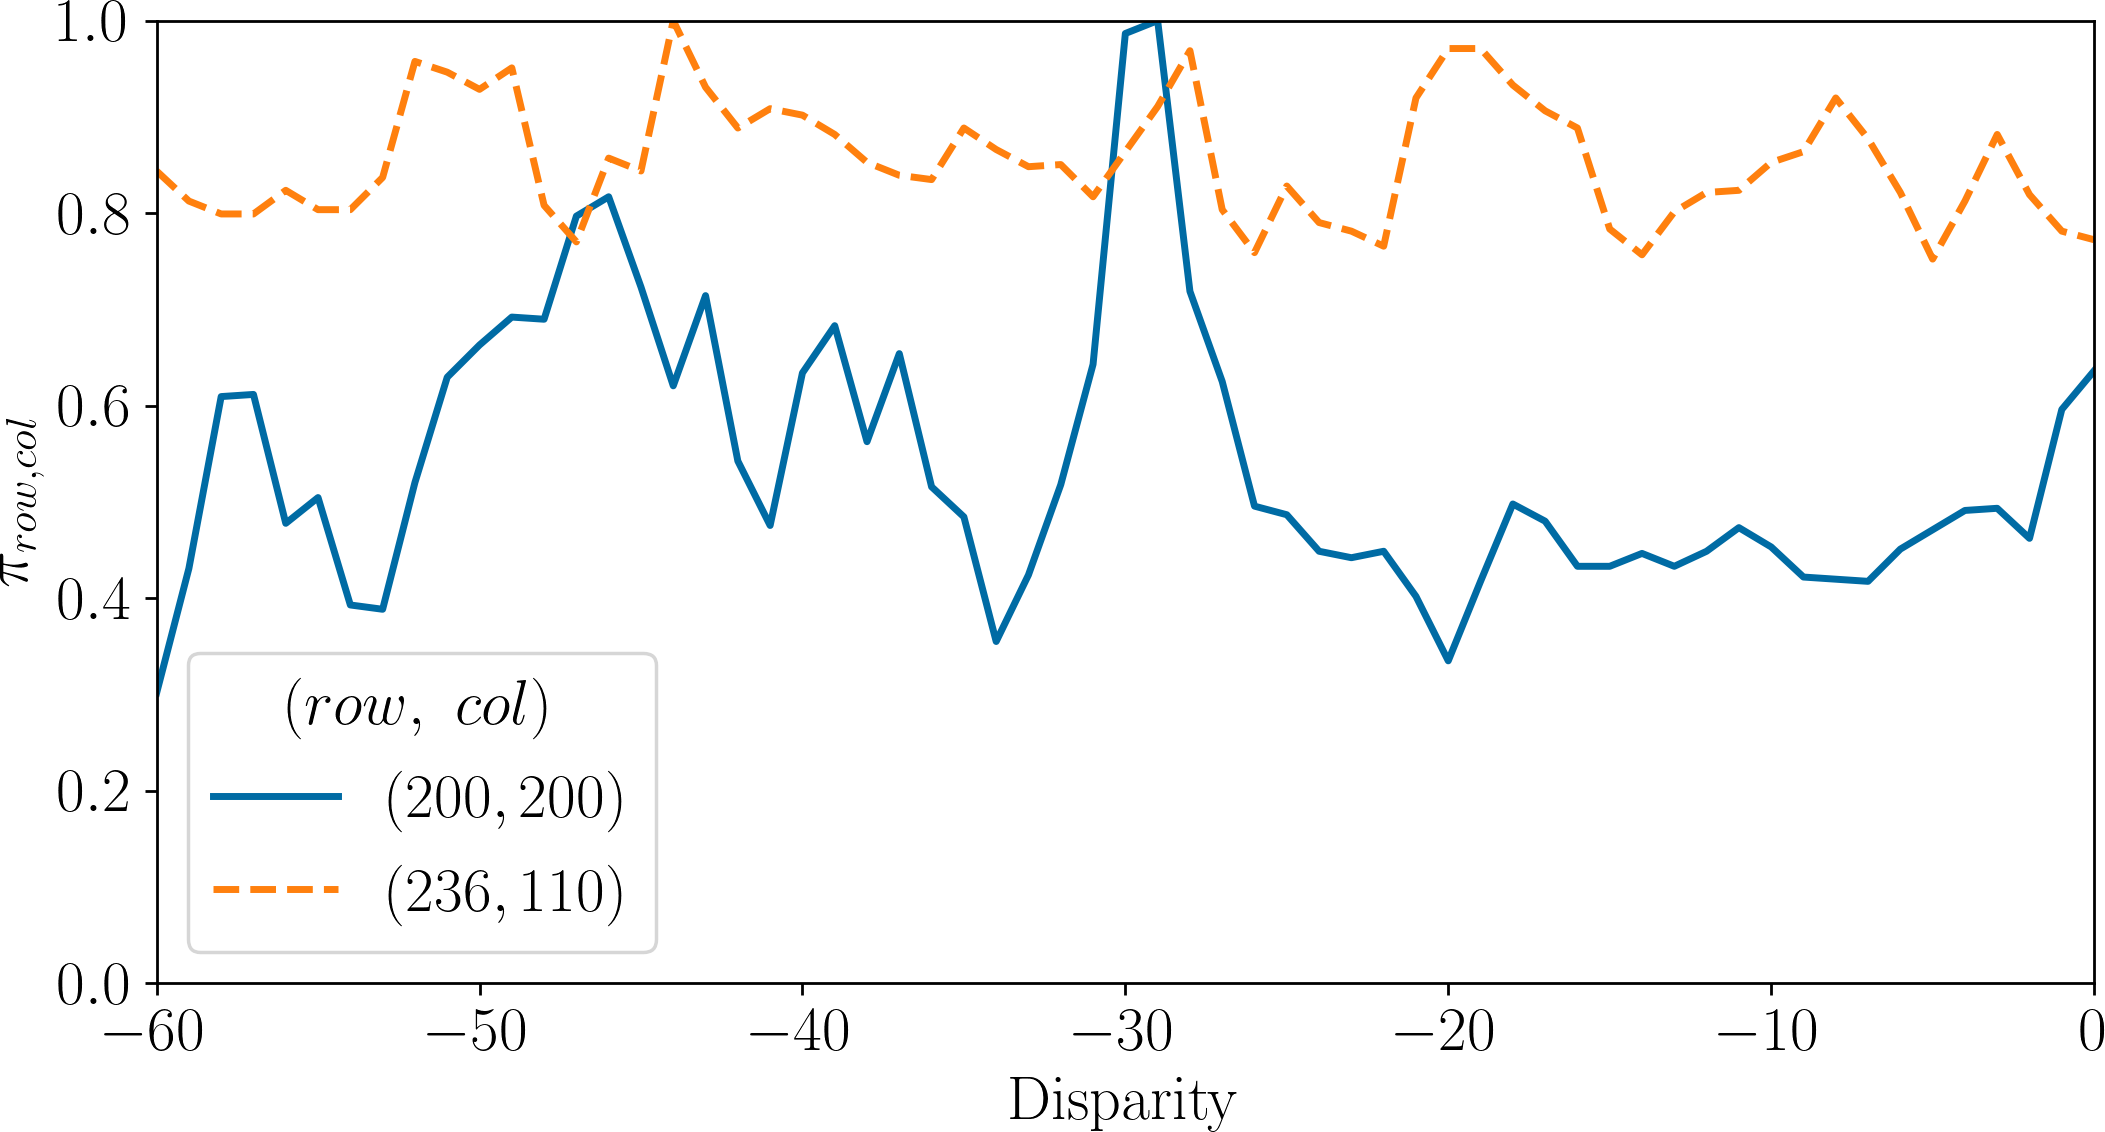
\includegraphics[width=\linewidth]{Images/Chap_5/cost_curve_possibility_distribution.png}
        \caption{Possibility distributions resulting from the cost curves}
        \label{fig:cost_curves_d}
    \end{subfigure}\hfill
    \caption{Transformation of cost curves (CENSUS + \acrshort{sgm} on Middlebury Cones) into possibility distributions. \Cref{fig:cost_curves_a} represents two cost curves that are normalized differently in \Cref{fig:cost_curves_b,fig:cost_curves_c}. \Cref{fig:cost_curves_d} uses the normalization of \Cref{fig:cost_curves_c} to create possibility distributions.}
    \label{fig:cost_curves_to_possibility}
\end{figure}

As stated previously, global extrema in \cref{eq:normalized_cost_curve} are employed to minimize the stretching effect when converting cost curves into possibility distributions. However, we also could have used the theoretical extrema of a cost curve instead. For instance, the CENSUS cost function on a $5\times5$ window provides values between $0$ and $C_{max}=24$. Adding \acrshort{sgm} regularization with penalty $P_2$ on $8$ directions yields cost volumes values between $0$ and $8\times(C_{max}+P_2)$ \cite{hirschmuller_accurate_2005}. However, this maximal cost is rarely attained in real case scenarios, and\commanue{je remplacerais and par therefore it} is too pessimistic and tends to over-compress the normalized cost curves. It is instead preferred to use global extrema of the cost volume for the normalization, as we suppose the best and worst match should have similar cost values across different scenes. This hypothesis is not restrictive for the images we consider in our stereo matching problem, as the size and diversity inside each scene lead to similar extrema. 

\subsection{From Possibilities to Disparity Confidence Intervals}
With the possibility distributions defined, our next objective is to establish a set of most possible disparities. We decided to aim for sets containing the true disparity $90\%$ of the time. This \( 90\%\) value was chosen following discussions with users and other experts working at CNES, IGN and more generally in the AI4GEO consortium\commanue{moi j'aurais introduit cette info avant dans l'intro et là tu peux le rappeler. Mais là c'est toi qui voit}. To define this set of most possible disparities, we compute the $\alpha$-cut (\cref{eq:alpha_cut}\commanue{tu fais un renvoi à l'équation, moi je renverrais à la définition. Bon c'est au même endroit de toute façon}) of the possibilities, or in other words, the set of all disparities $D_\alpha$ whose possibility is superior than $\alpha$:
\begin{align}
    D_\alpha=\{~ d ~|~ \pi_{row,col}(d)\geqslant\alpha\}\label{eq:set_of_possible_disparities}
\end{align}
By looking at possibility distributions obtained from different cost curves for which we know the true disparity, we first fixed the value $\alpha$ at $0.9$. In depth study of this parameter will be tested later, in order to see if it depends on the cost function, the type of scene considered, and to provide general guidelines on its optimal value. In the following, when the value of $\alpha$ is not specified, it will always be set at $0.9$. The fact that its value is the same as the $90\%$ confidence objective is a coincidence and one should not suppose that $\alpha$ and the confidence objective should be the same. Indeed raising the $\alpha$ value would decrease the size of the set $D_\alpha$ and therefore decrease the proportion of sets containing the true disparity, \ie the global confidence rate of intervals. \Cref{fig:disparity_intervals_a,fig:disparity_intervals_b} graphically represent $D_\alpha$ for the cost curves of \Cref{fig:cost_curves_to_possibility}.

\begin{remark}
    We are modelling the epistemic uncertainty of the cost curves using possibility distributions. In the rest of this chapter, we use a possibility distribution for each cost curve because we think it is a correct model in itself for the uncertainty we encounter. It is however possible to have a probabilistic interpretation of possibilities, which we will share in this remark as it may be of interest for people thinking the underlying uncertainty can be modeled by probabilities.
    
    We saw in \cref{eq:credal_set_possibility} from \Cref{chap:representation_of_uncertainty} that one way of interpreting $\pi_{row,col}$ is that it defines a set of probability distributions, \ie a credal set $\M$. We can also define $D_\alpha$ using this set $\M$, as:
    \begin{align}
        D_\alpha=\{~ d ~|~ \exists P\in\M ~\st~ P(d)\geqslant \alpha\}
    \end{align}
    or in plain words, $D_\alpha$ is the set of all disparities $d$ for which there exists a probability in $\M$ whose value is greater than $\alpha$ for $d$. We will not rely on this interpretation in the rest of this chapter, and instead only reason in terms of possibilities.
\end{remark}

\todoroman{Figure montrant différentes courbes de coût transformées, CENSUS MCCNN}

\Cref{eq:set_of_possible_disparities} defines a set of disparities $D_\alpha$ which is not necessarily convex. We will rather consider confidence disparity intervals $I_\alpha$ deduced from $D_\alpha$ in the rest of this chapter:
\begin{align}
    I_\alpha = [\underline{I}_\alpha,~\overline{I}_\alpha]=[\min D_\alpha, ~\max D_\alpha]\label{eq:confidence_disparity_intervals}
\end{align}
\Cref{fig:disparity_intervals_c,fig:disparity_intervals_d} graphically represent how $I_\alpha$ is determined for the two possibility distributions of the cost curves in \Cref{fig:cost_curves_to_possibility}. In the rest of this section, we will not make any distinction between disparity confidence intervals, disparity intervals, confidence intervals or simply intervals. A disparity interval is the convex envelope of its disparity set $D_\alpha$, which is a conservative approach as observed in \Cref{fig:disparity_intervals_b,fig:disparity_intervals_d}.

Considering intervals thus presents the advantage of working with convex sets and only requiring two scalars to describe the set. Users of the \acrshort{dsm}s produces by stereo photogrammetry are also used to consider confidence intervals \cite{oksanen_digital_2006, wang_robust_2015, panagiotakis_validation_2018, deschamps-berger_apport_2021, hugonnet_uncertainty_2022}. This will also facilitate further processing in the rest of the stereo pipeline, as we only need to take into account $2$ bounds to characterize the possible disparities, instead of a set of arbitrary shape.

\begin{figure}
    \centering
    \begin{subfigure}[t]{0.47\linewidth}
        \centering
        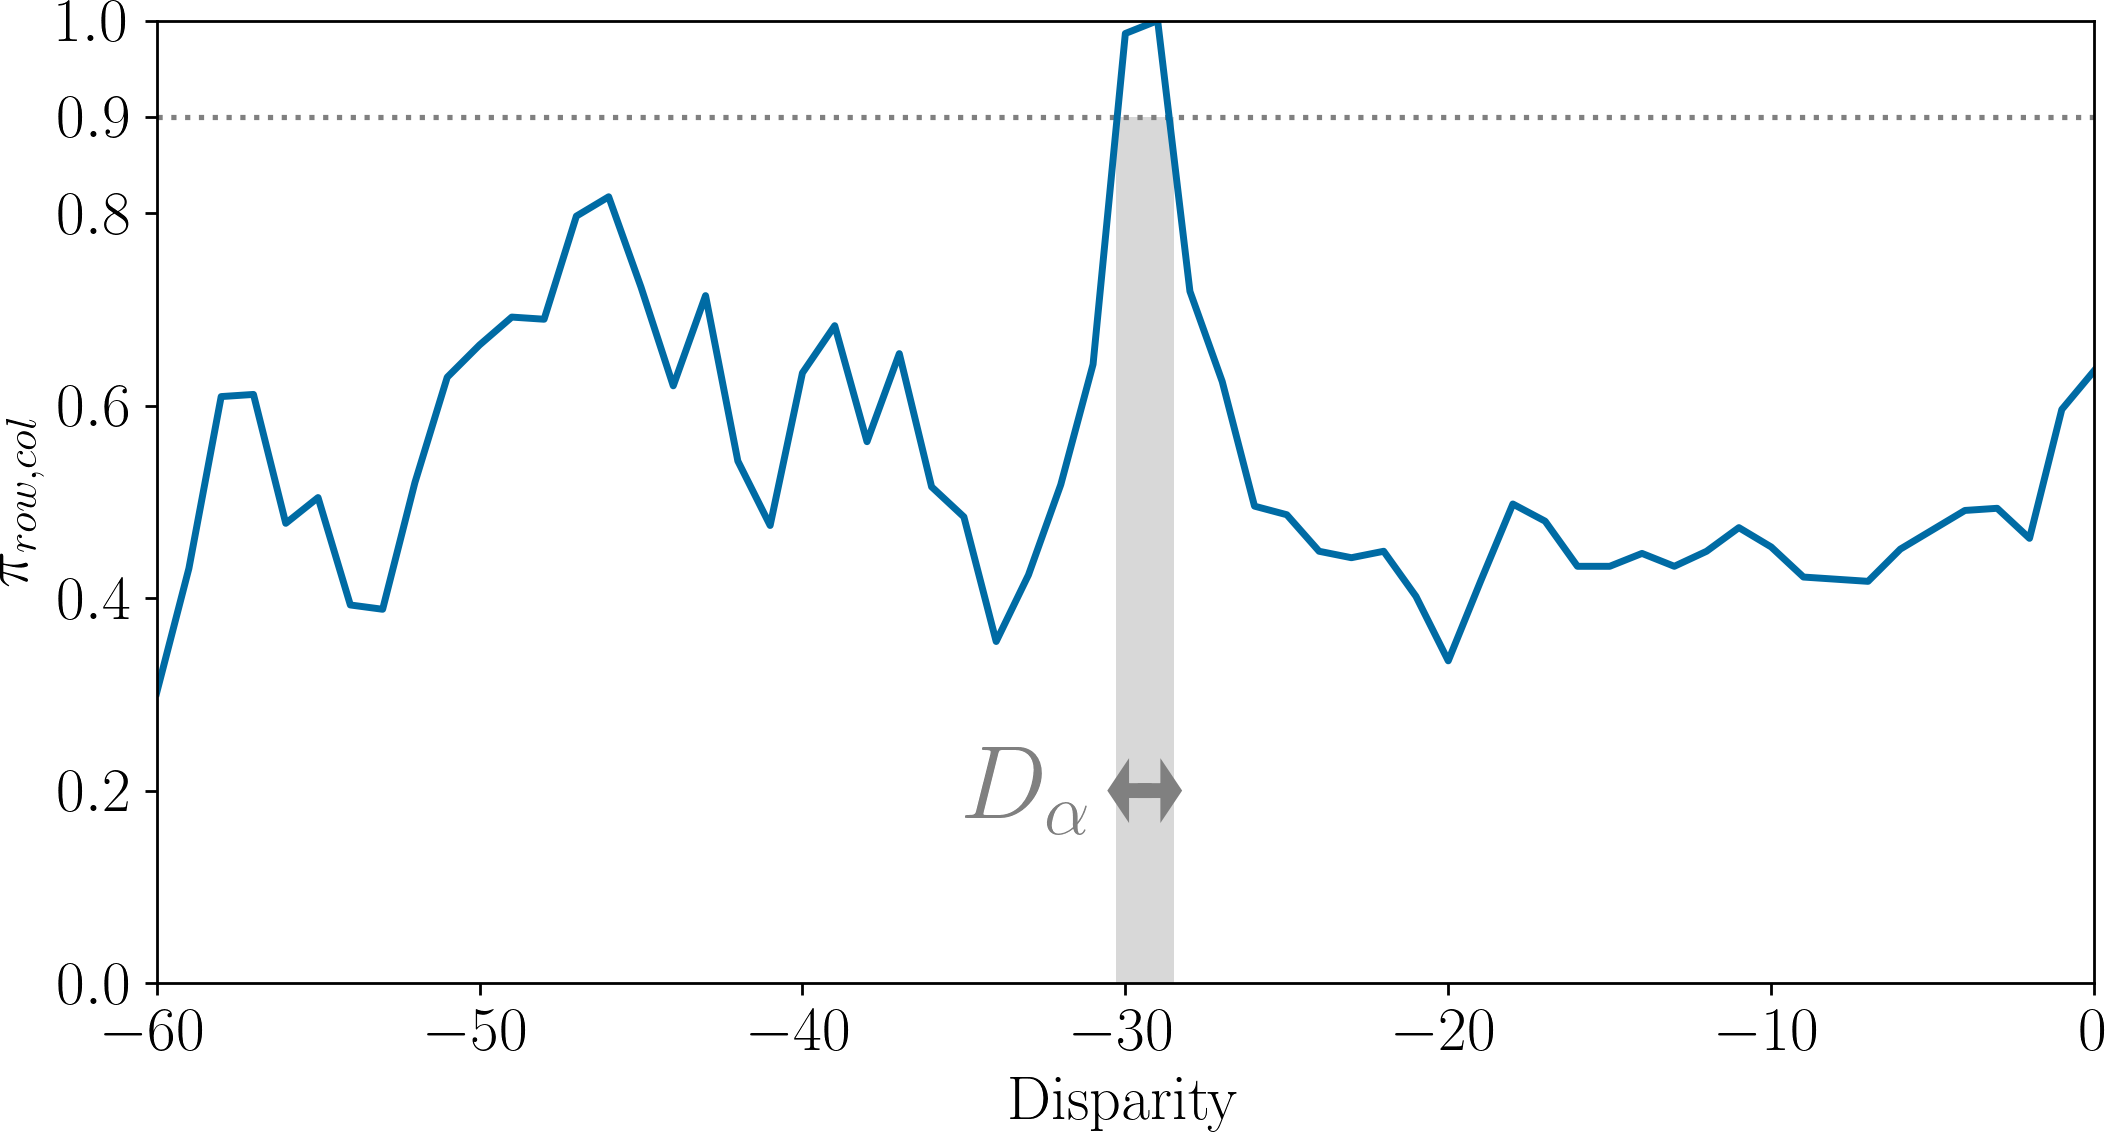
\includegraphics[width=\linewidth]{Images/Chap_5/disparity_interval_1.png}
        \caption{$D_\alpha$ for the blue possibility of \Cref{fig:cost_curves_d}}
        \label{fig:disparity_intervals_a}
    \end{subfigure}\hfill
    \begin{subfigure}[t]{0.47\linewidth}
        \centering
        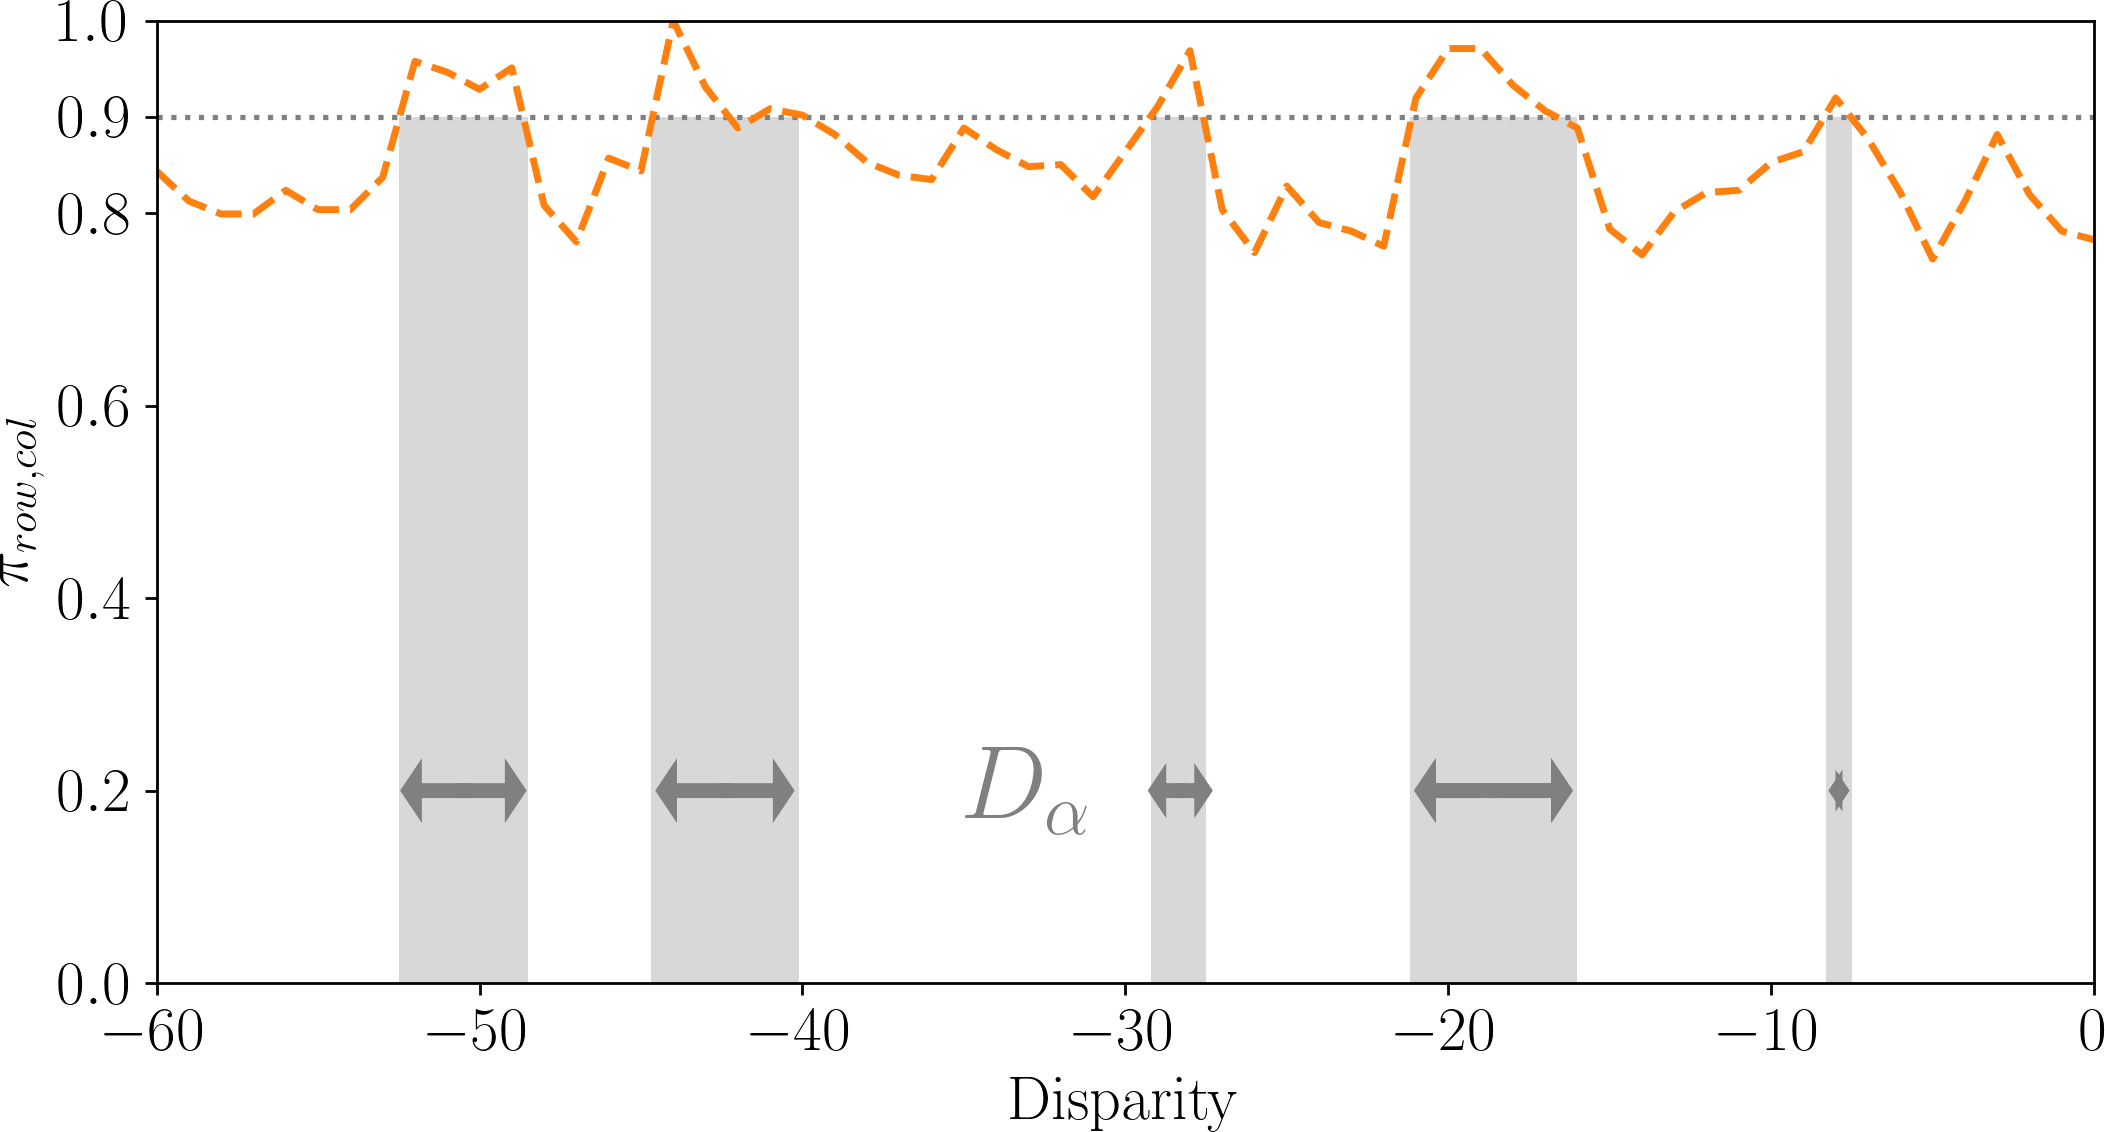
\includegraphics[width=\linewidth]{Images/Chap_5/disparity_interval_2.png}
        \caption{$D_\alpha$ for the orange possibility of \Cref{fig:cost_curves_d}}
        \label{fig:disparity_intervals_b}
    \end{subfigure}
    \begin{subfigure}[t]{0.47\linewidth}
        \centering
        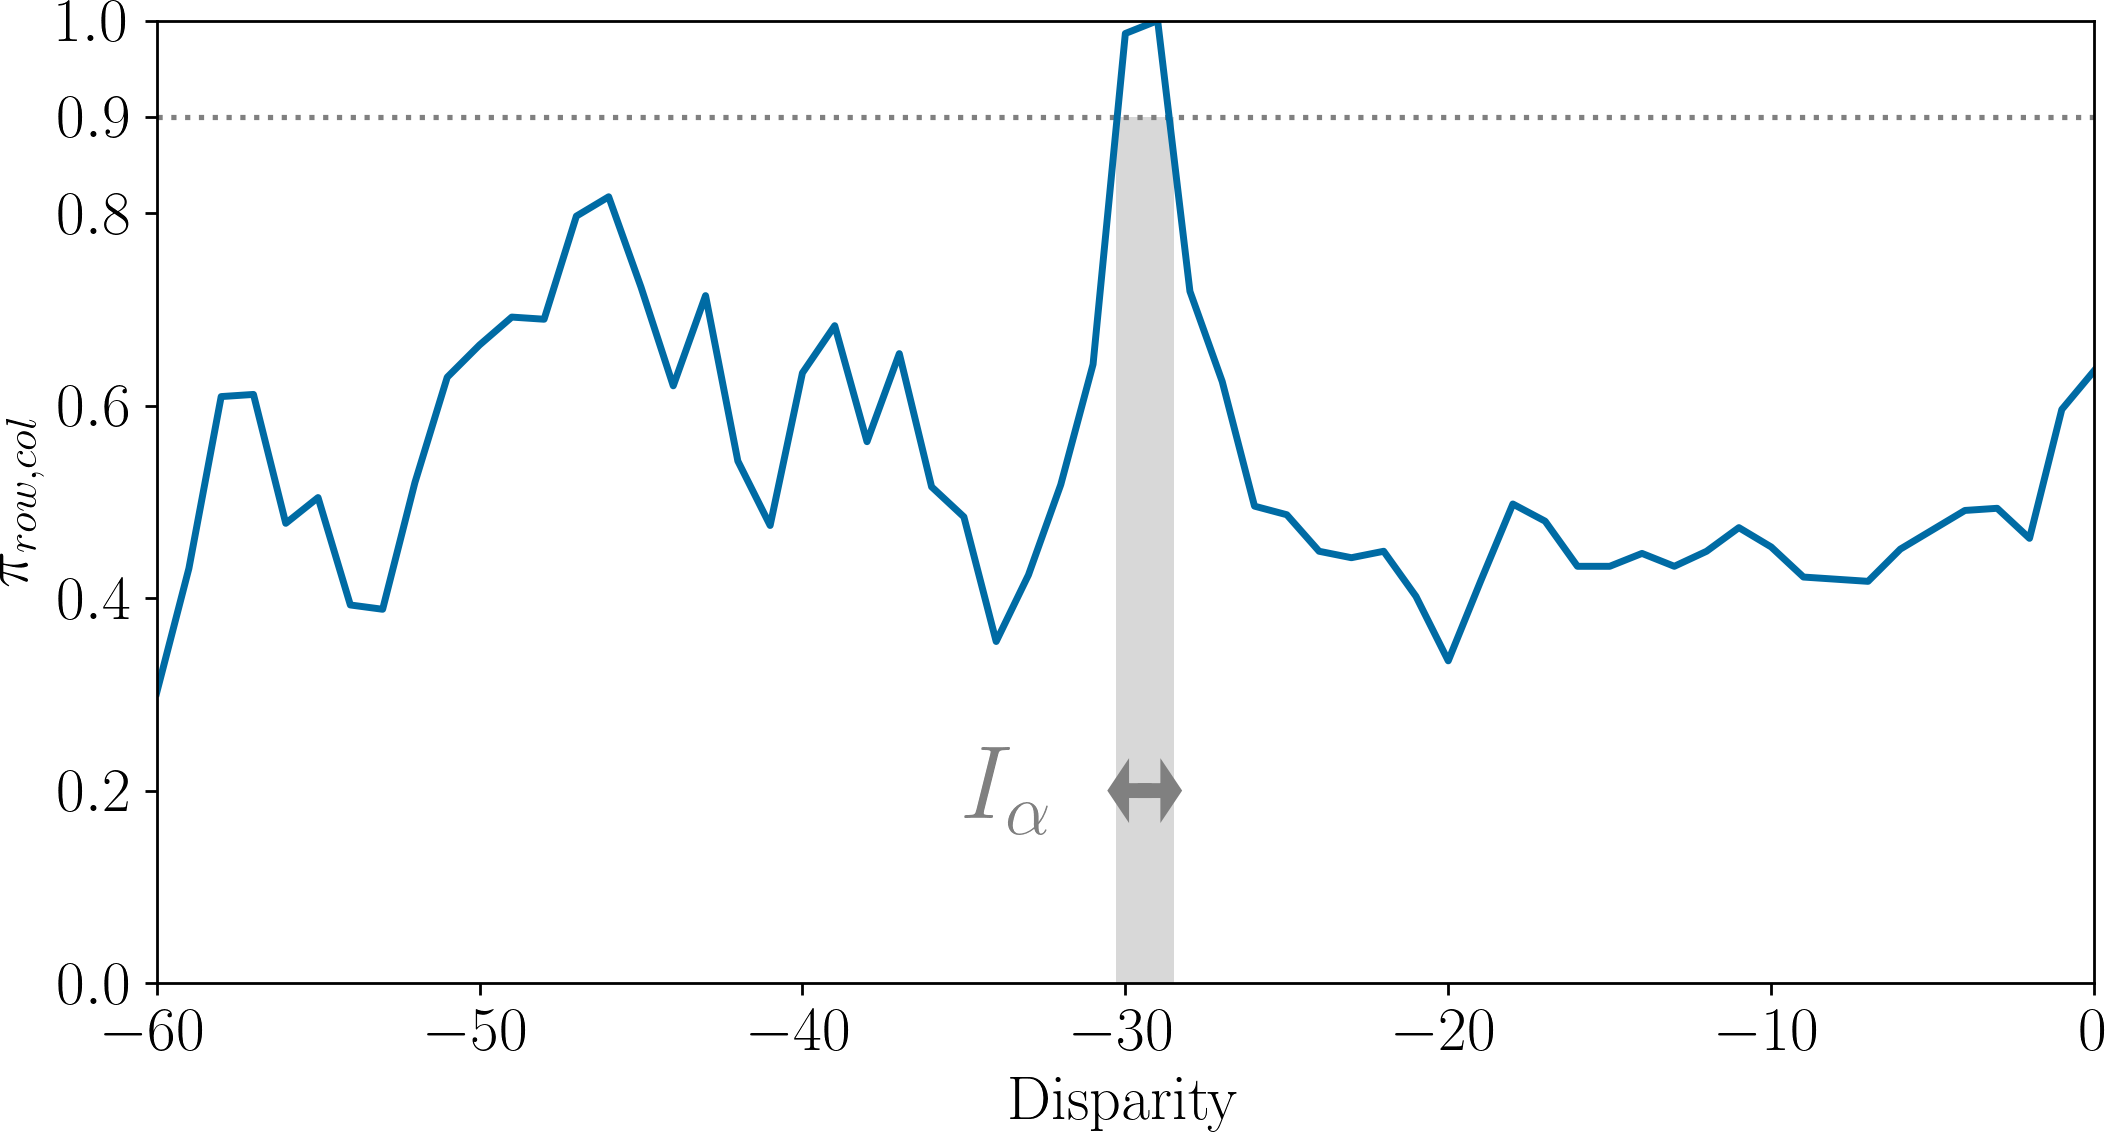
\includegraphics[width=\linewidth]{Images/Chap_5/disparity_interval_3.png}
        \caption{$I_\alpha$ for the blue possibility of \Cref{fig:cost_curves_d}}
        \label{fig:disparity_intervals_c}
    \end{subfigure}\hfill
    \begin{subfigure}[t]{0.47\linewidth}
        \centering
        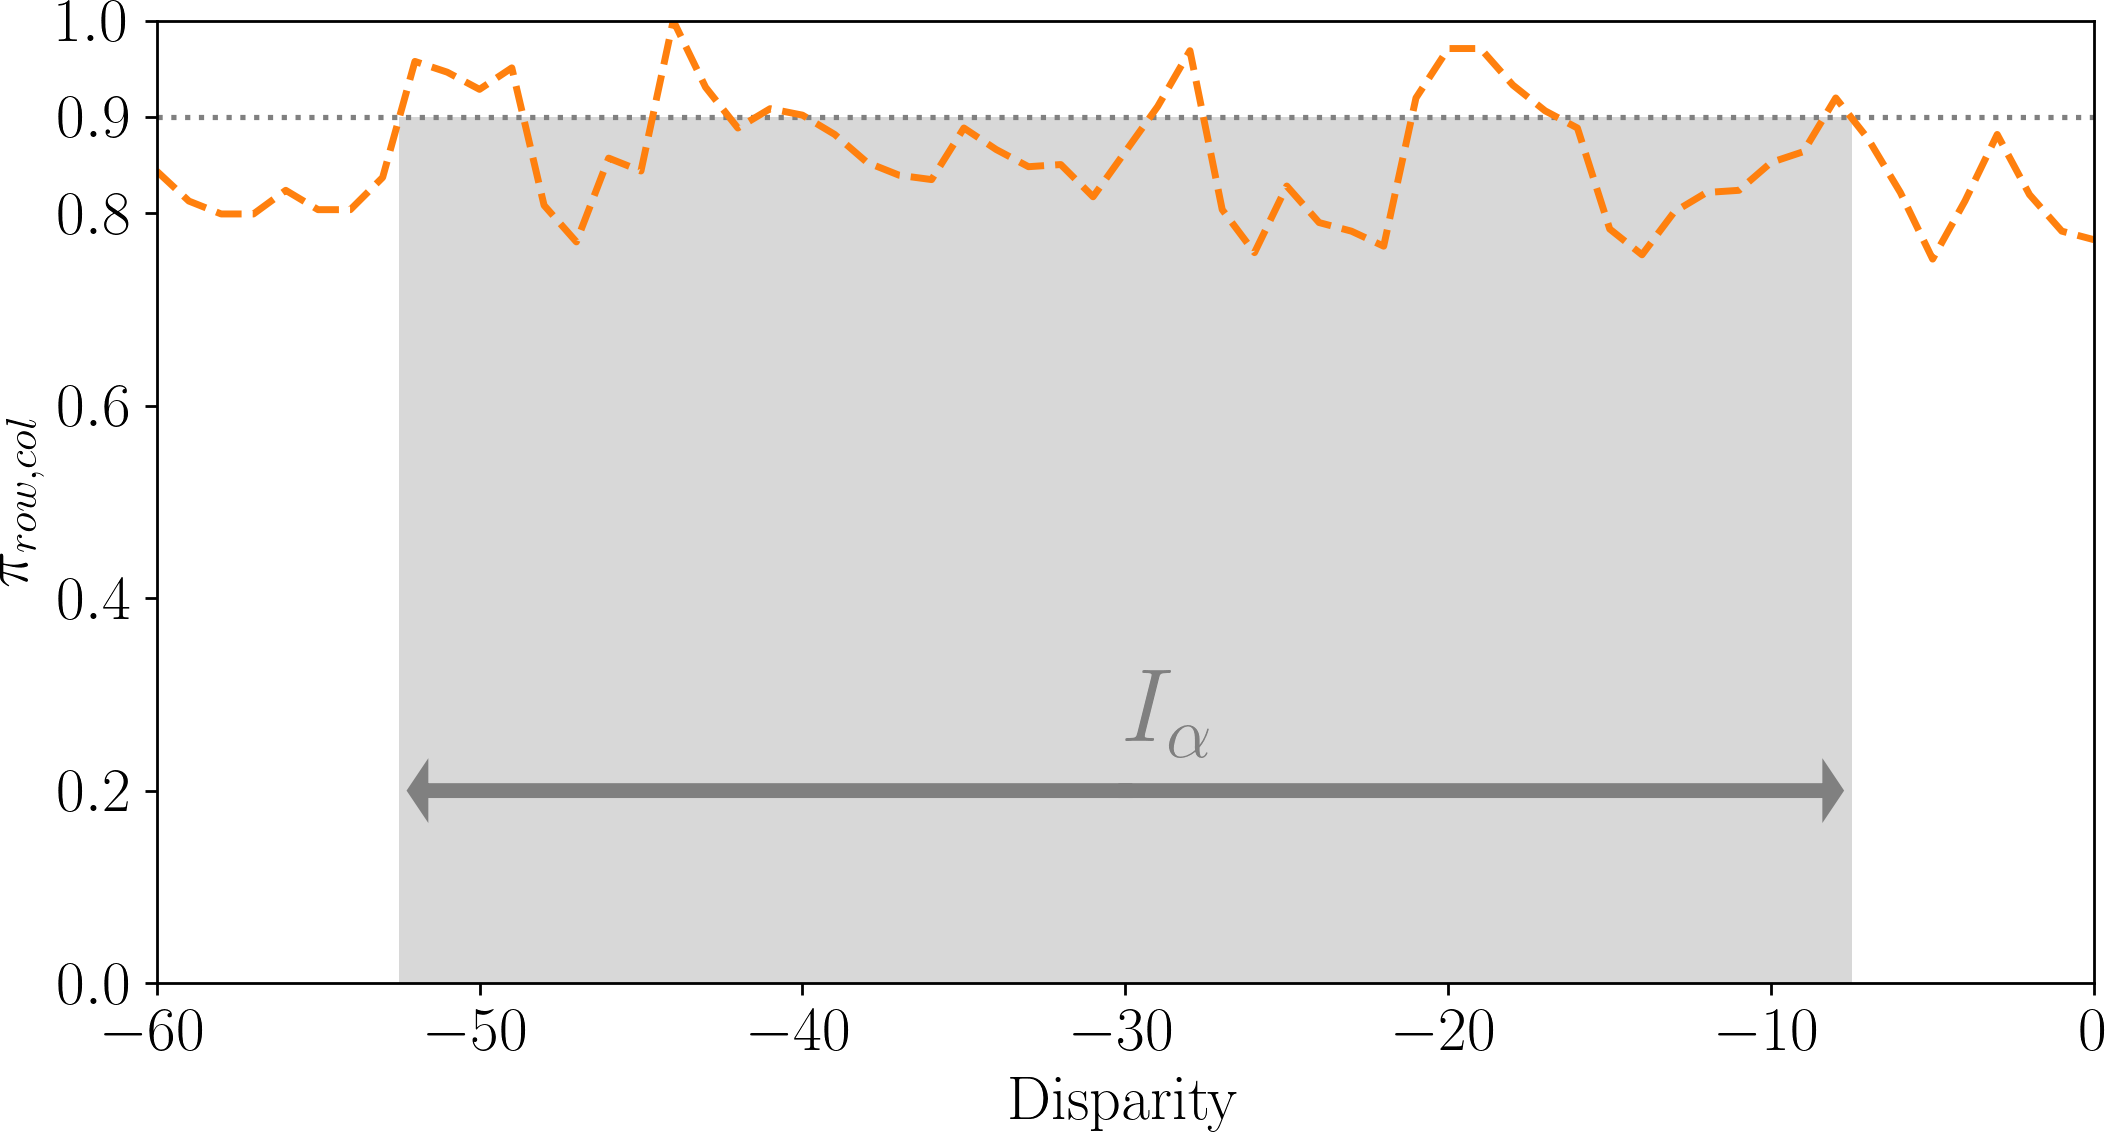
\includegraphics[width=\linewidth]{Images/Chap_5/disparity_interval_4.png}
        \caption{$I_\alpha$ for the orange possibility of \Cref{fig:cost_curves_d}}
        \label{fig:disparity_intervals_d}
    \end{subfigure}\hfill
    \caption{Set of possible disparities $D_\alpha$ and disparity intervals $I_\alpha$ with the same cost curves as in  \Cref{fig:cost_curves_to_possibility}, with $\alpha=0.9$. \Cref{fig:disparity_intervals_a,fig:disparity_intervals_b} represent the set of possible disparities $D_\alpha$ from \cref{eq:set_of_possible_disparities} in gray. \Cref{fig:disparity_intervals_c,fig:disparity_intervals_d} represent disparity intervals $I_\alpha$ from \cref{eq:confidence_disparity_intervals} in gray. There is no difference between $D_\alpha$ and $I_\alpha$ for the blue curve, contrary to the orange dashed curve.}
    \label{fig:disparity_sets_and_intervals}
\end{figure}

To qualitatively evaluate the behaviour of disparity confidence intervals $I_\alpha$, we will look at their values for different pixels of the same row. The rows considered are presented in \Cref{fig:cones_with_rows}: the upper row ($80$) is smaller so more details can be observed, while other rows provide broader estimations of the intervals. By construction, $I_\alpha$ will always contain the predicted disparity $\tilde{d}$, and we want to see if it can contain the true disparity $d_{true}$ even when the predicted disparity is far from it. \Cref{fig:intervals_ambiguous_row_80_1,fig:intervals_ambiguous_row_180_1,fig:intervals_ambiguous_row_240_1,fig:intervals_ambiguous_row_290_1} 

\begin{figure}
    \centering
    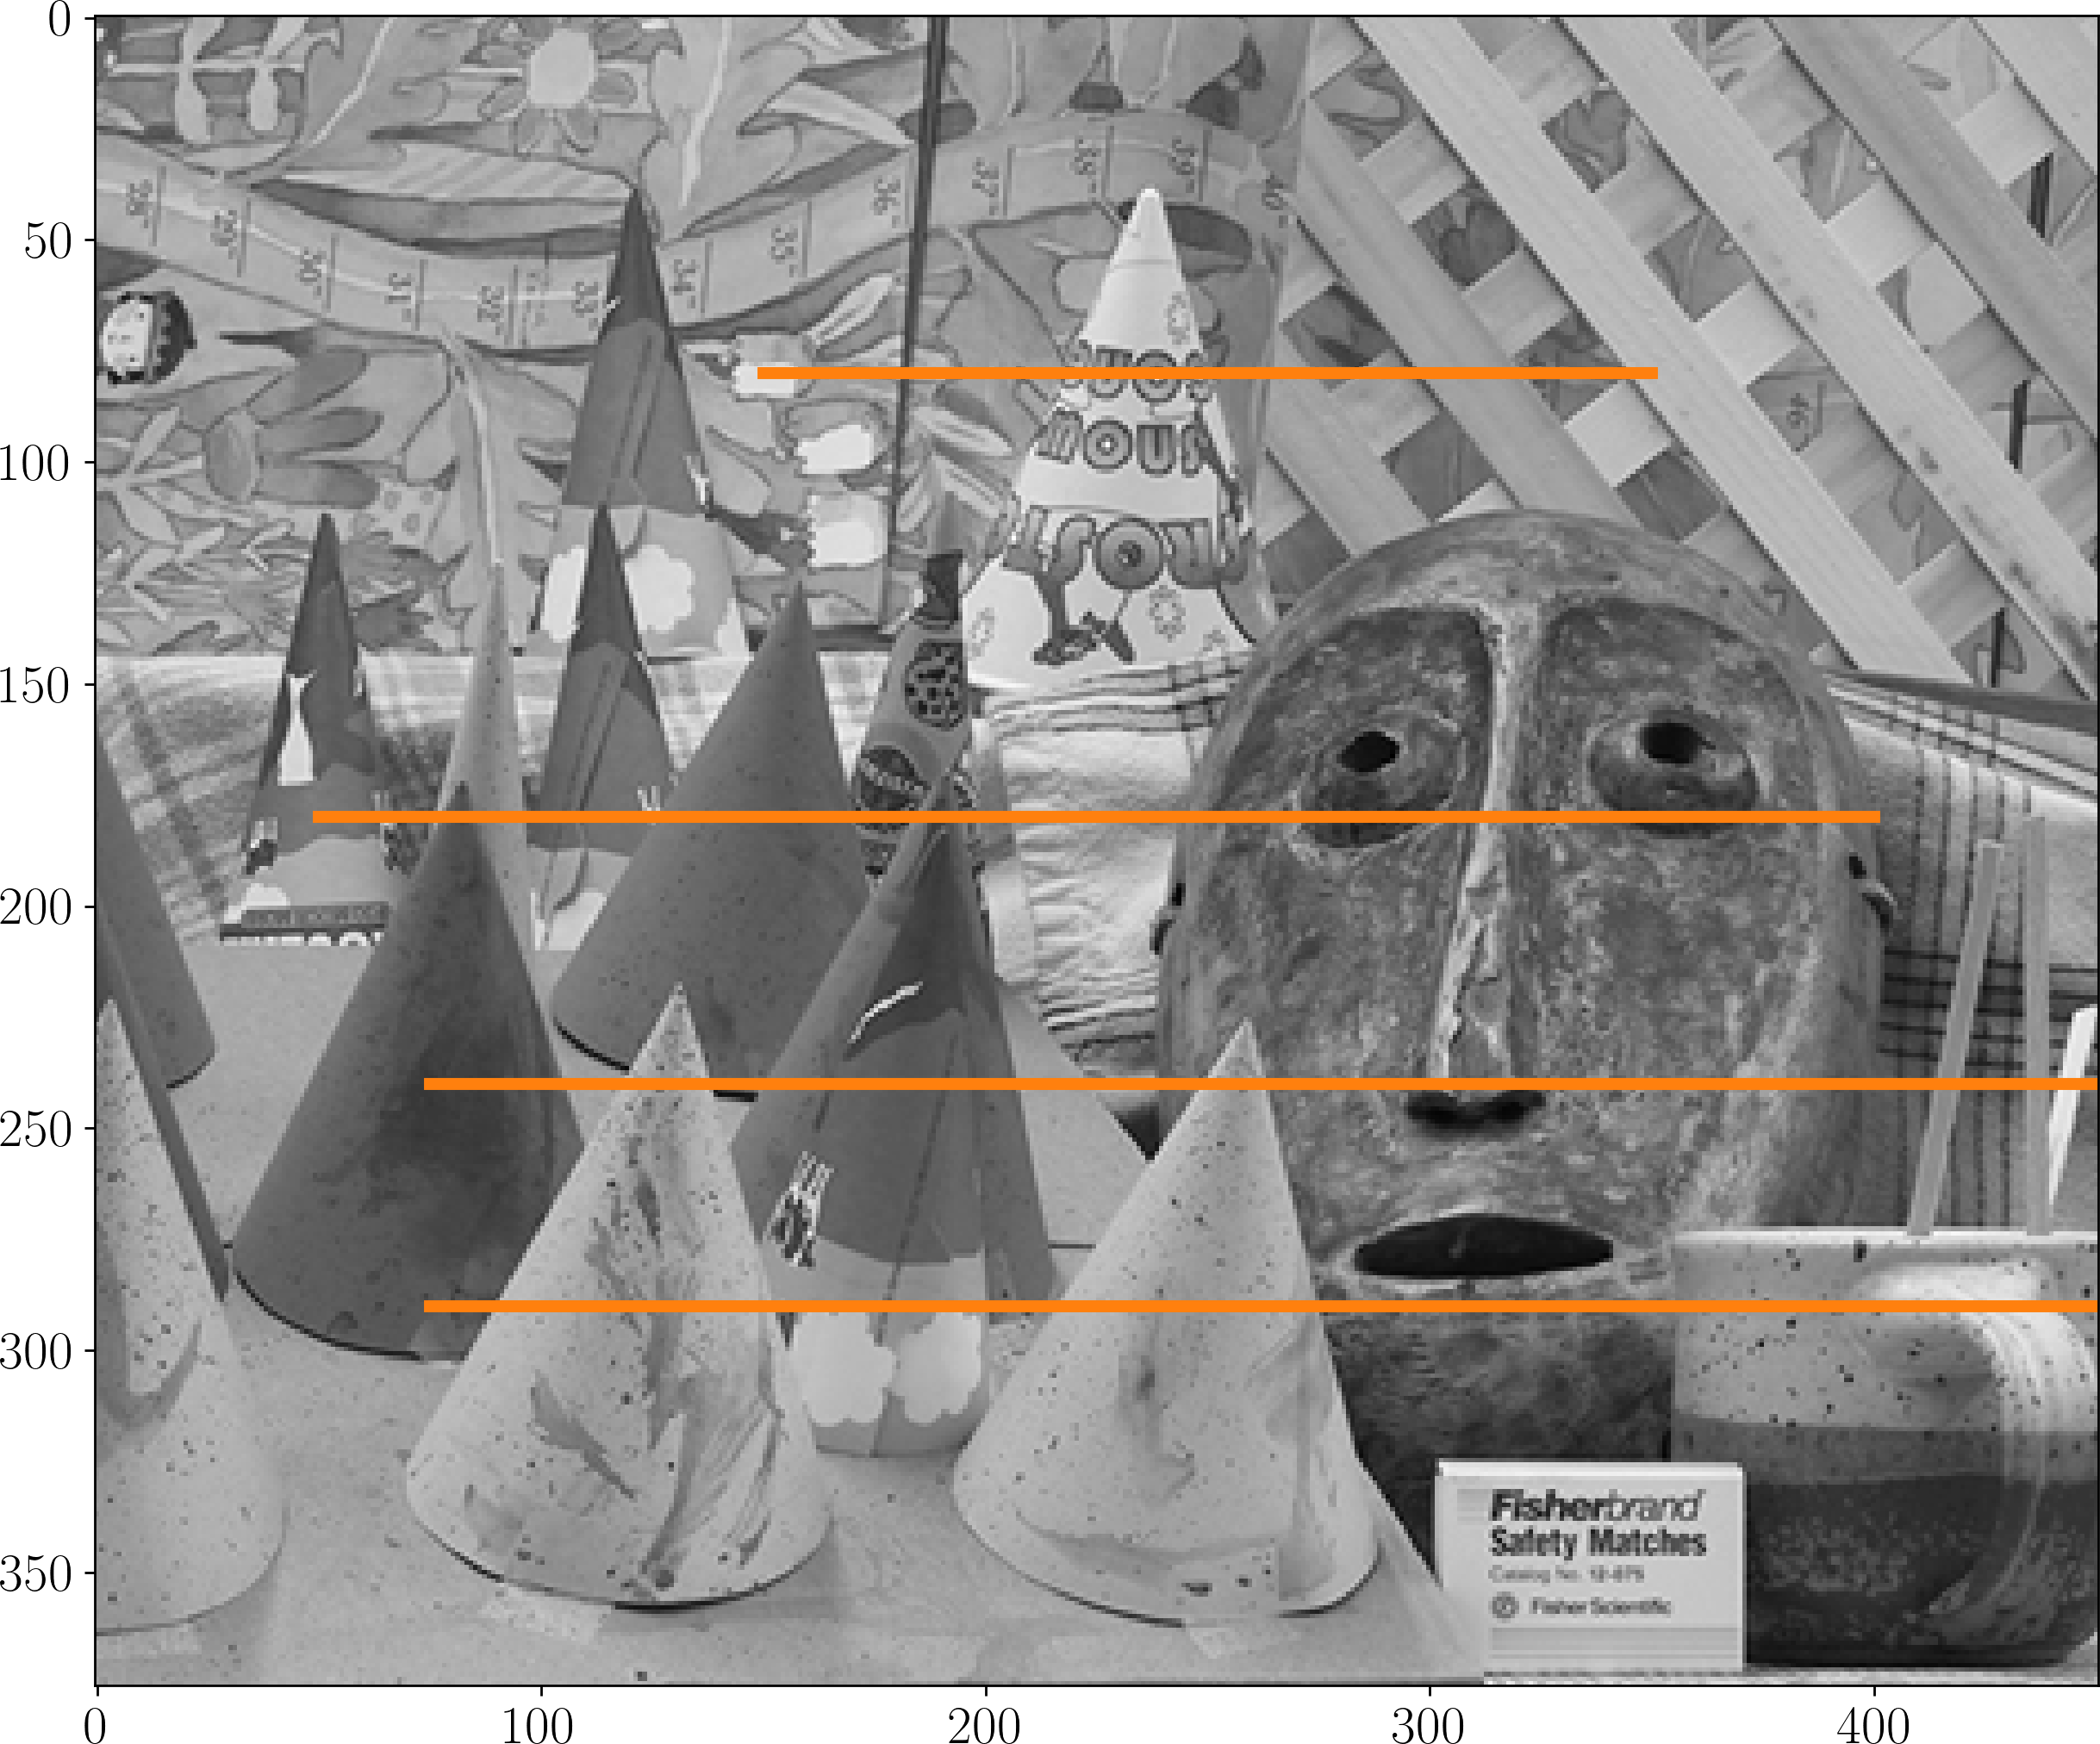
\includegraphics[width=0.5\linewidth]{Images/Chap_5/cones_with_rows.png}
    \caption{Left stereo image from Middlebury Cones. Disparity intervals $I_\alpha$ along orange lines are detailed in \Cref{fig:intervals_ambiguous_row_80,fig:intervals_ambiguous_row_180,fig:intervals_ambiguous_row_240,fig:intervals_ambiguous_row_290}}
    \label{fig:cones_with_rows}
\end{figure}

\begin{figure}
    \centering
    \begin{subfigure}[t]{0.8\linewidth}
        \centering
        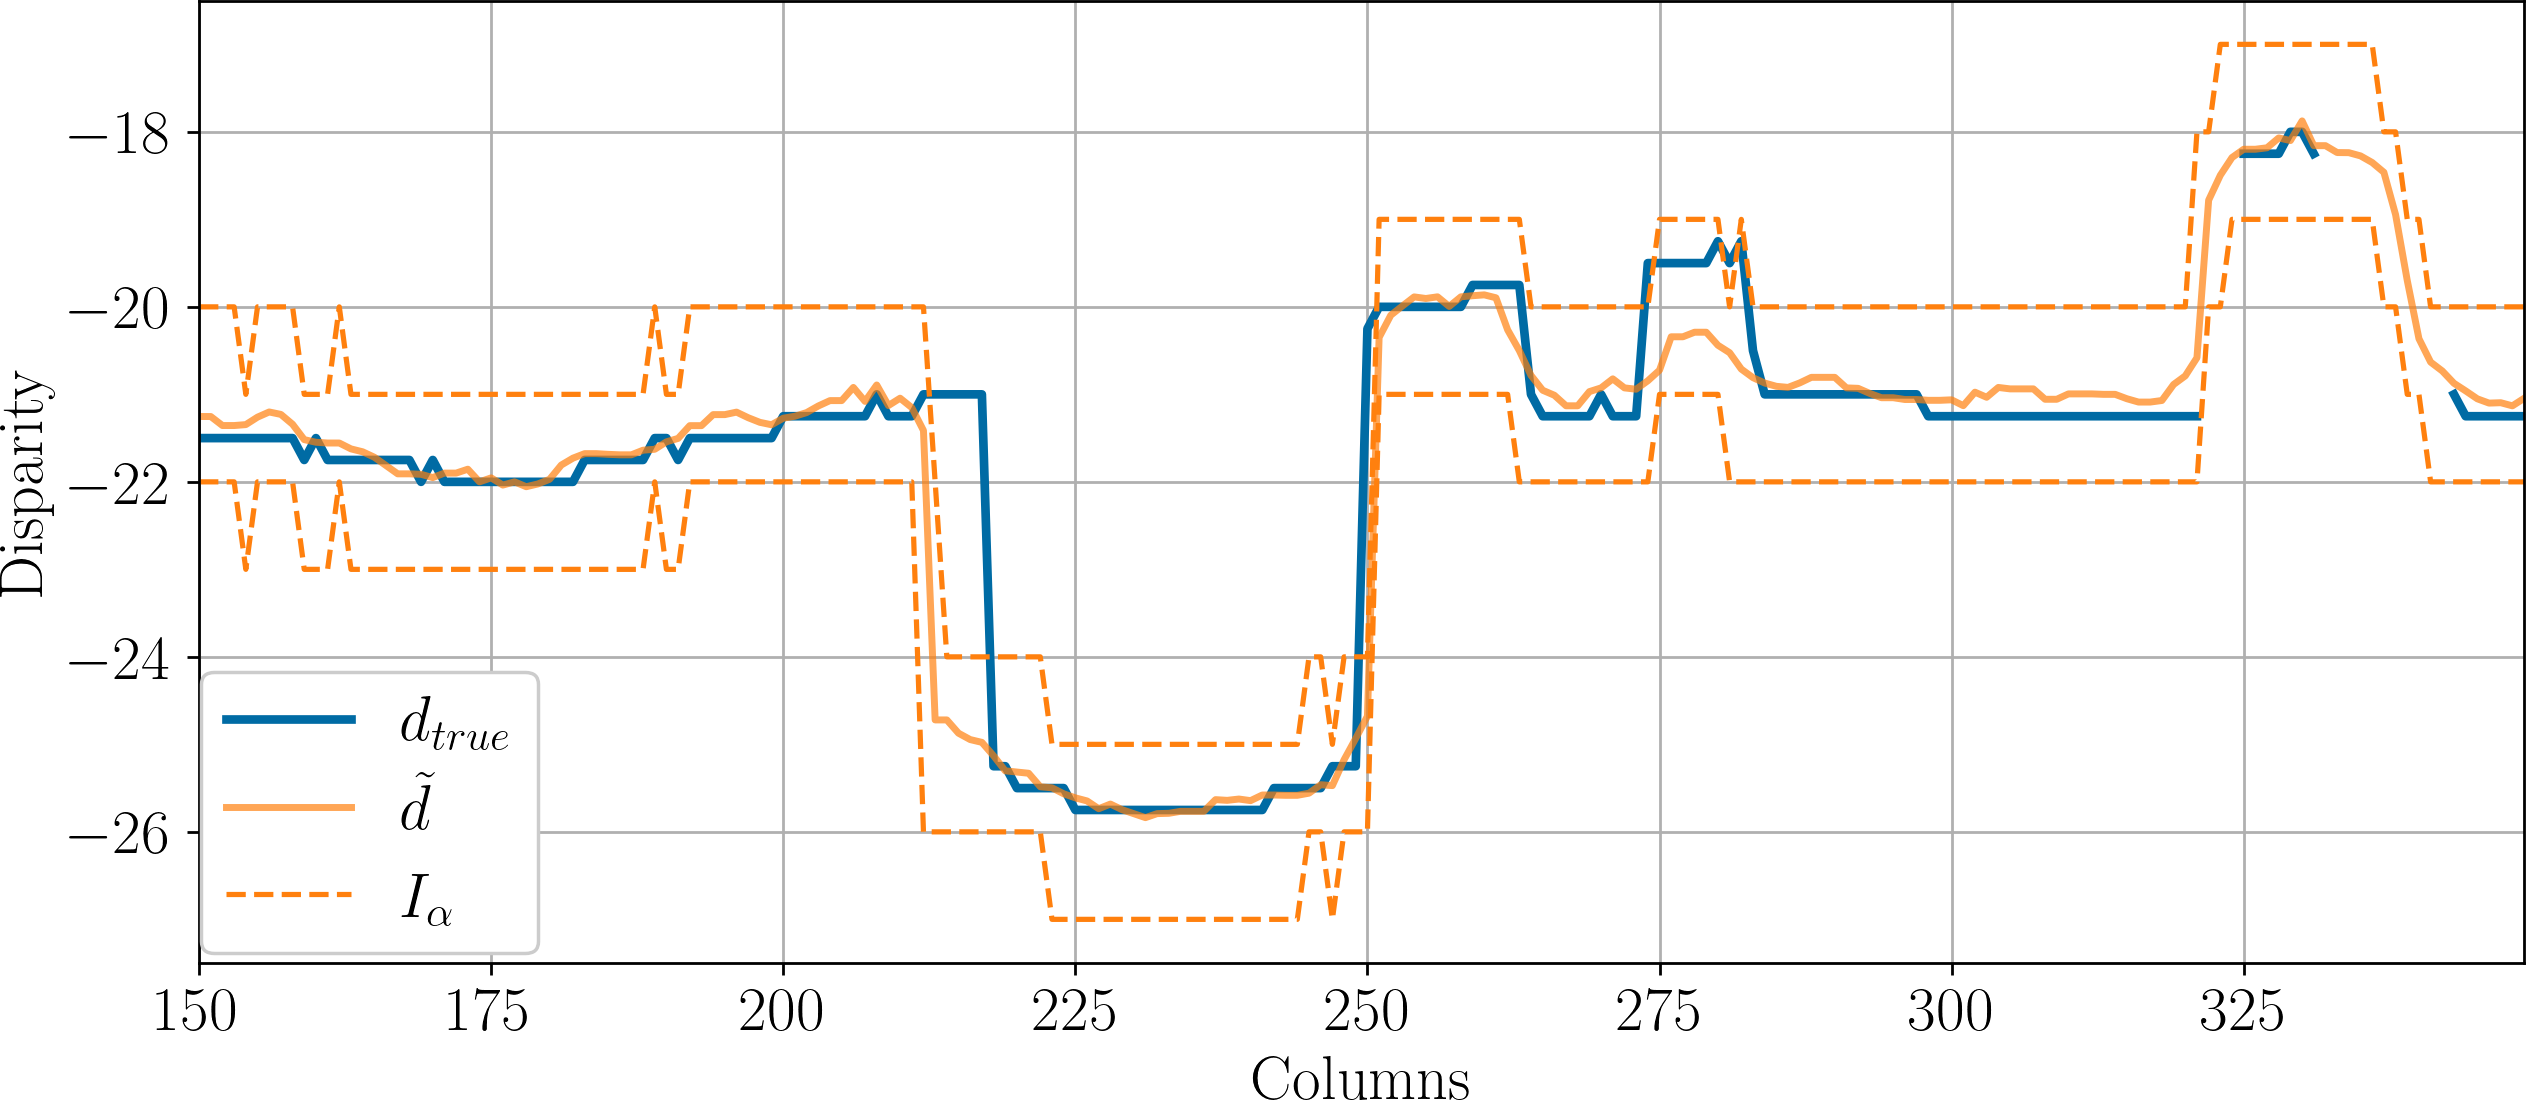
\includegraphics[width=\linewidth]{Images/Chap_5/intervals_ambiguous_area_row_80_1.png}
        \caption{$I_\alpha$ without regularization in low confidence areas}
        \label{fig:intervals_ambiguous_row_80_1}
    \end{subfigure}\hfill
    \begin{subfigure}[t]{0.8\linewidth}
        \centering
        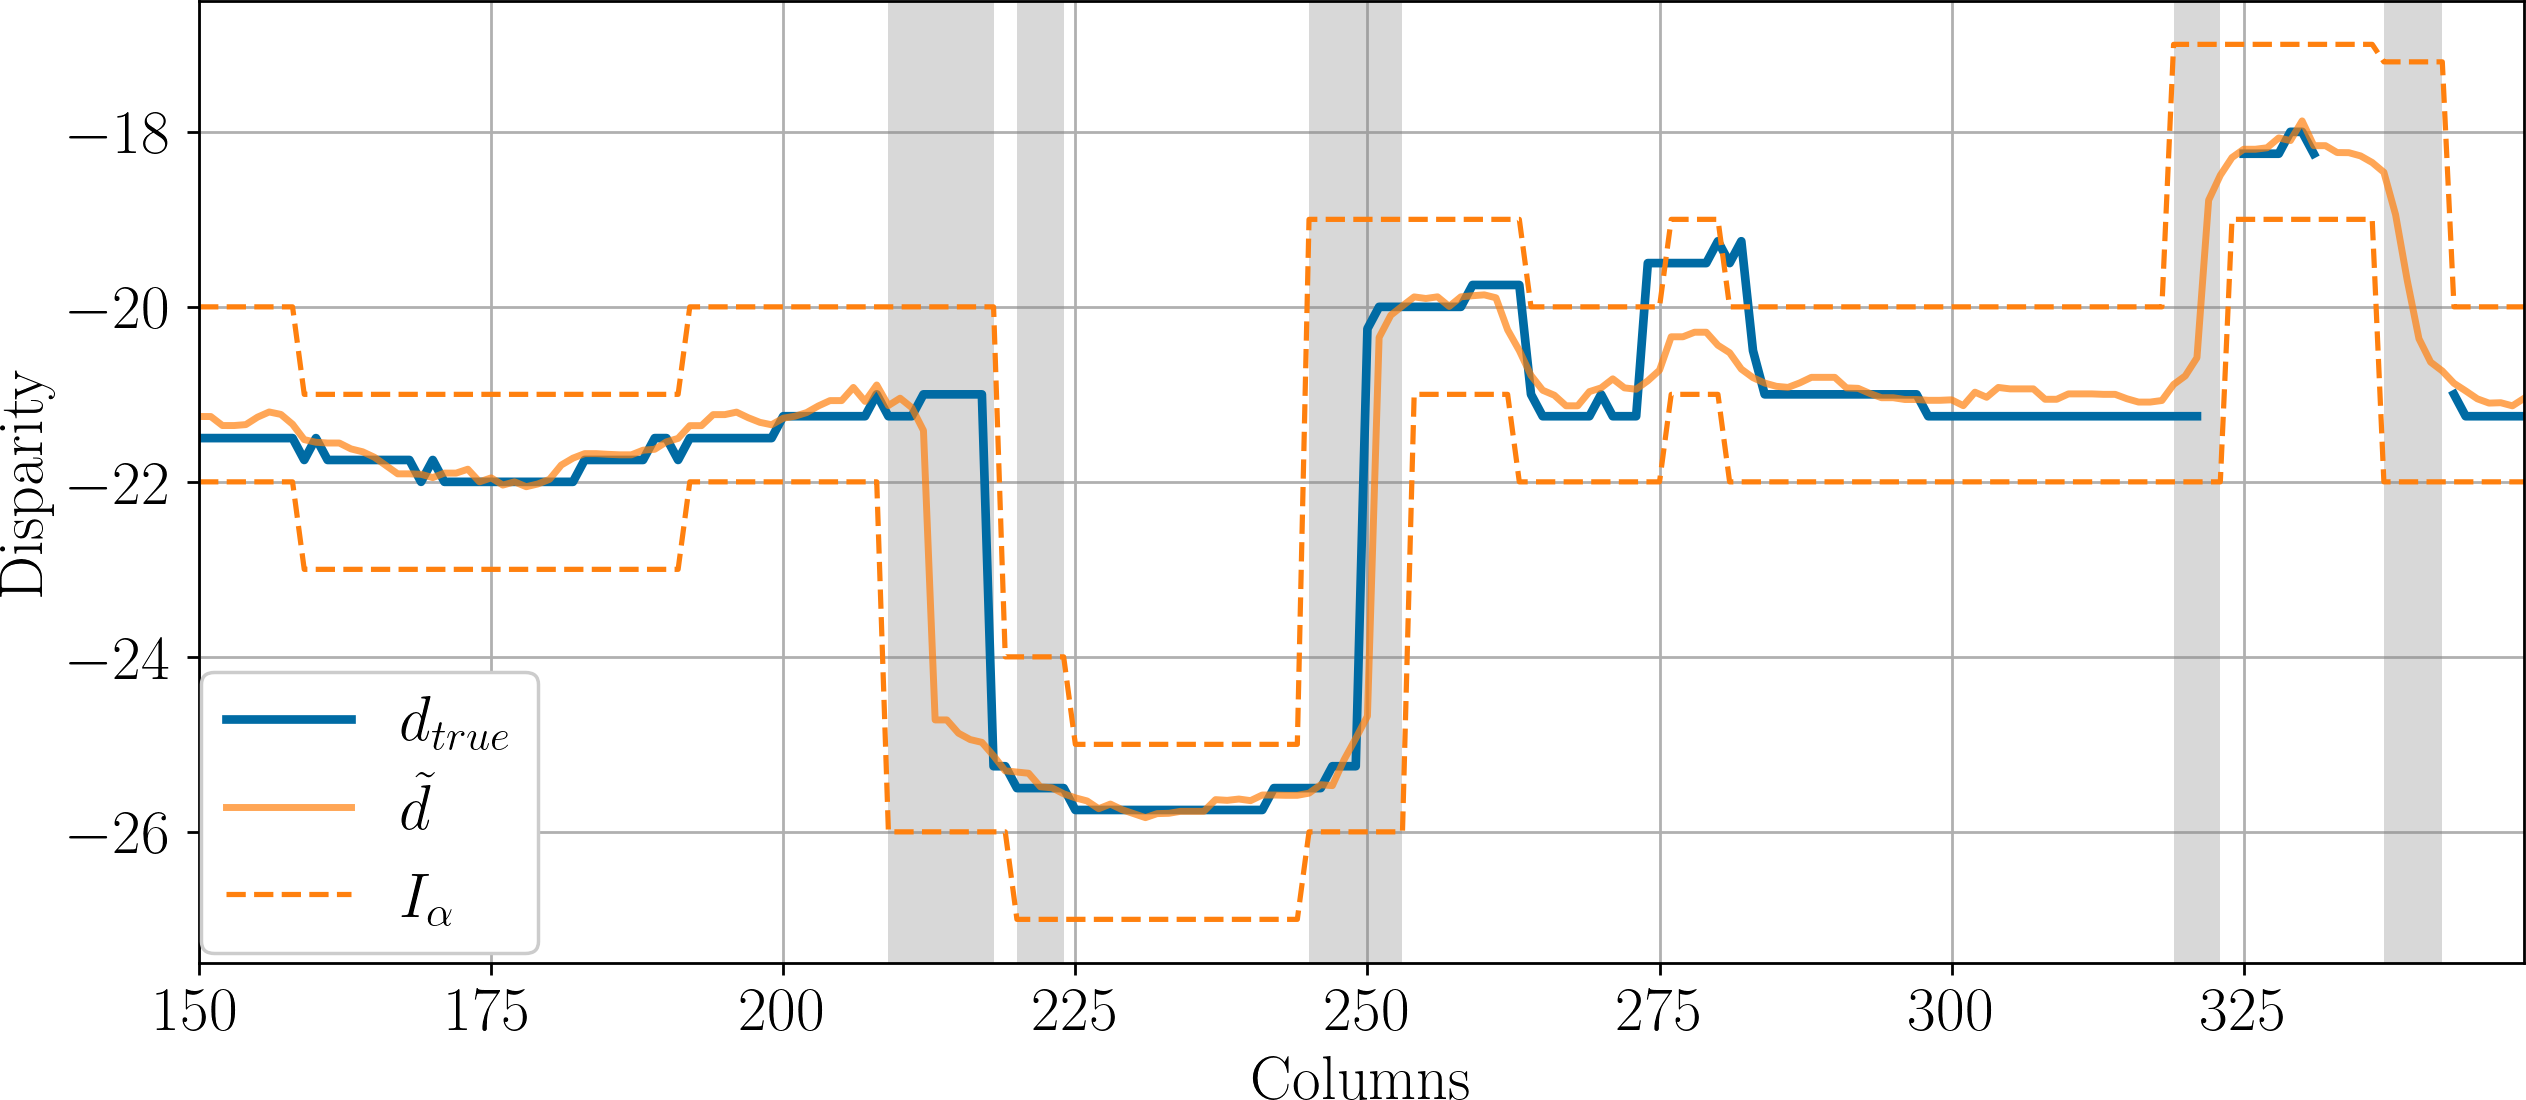
\includegraphics[width=\linewidth]{Images/Chap_5/intervals_ambiguous_area_row_80_2.png}
        \caption{$I_\alpha$ with regularization in low confidence areas}
        \label{fig:intervals_ambiguous_row_80_2}
    \end{subfigure}
    \caption{$I_\alpha$ with and without regularization in low confidence area, for row $80$ of the image of \Cref{fig:cones_with_rows}. Low confidence areas are indicated by the gray areas.}
    \label{fig:intervals_ambiguous_row_80}
\end{figure}
\begin{figure}
    \centering
    \begin{subfigure}[t]{\linewidth}
        \centering
        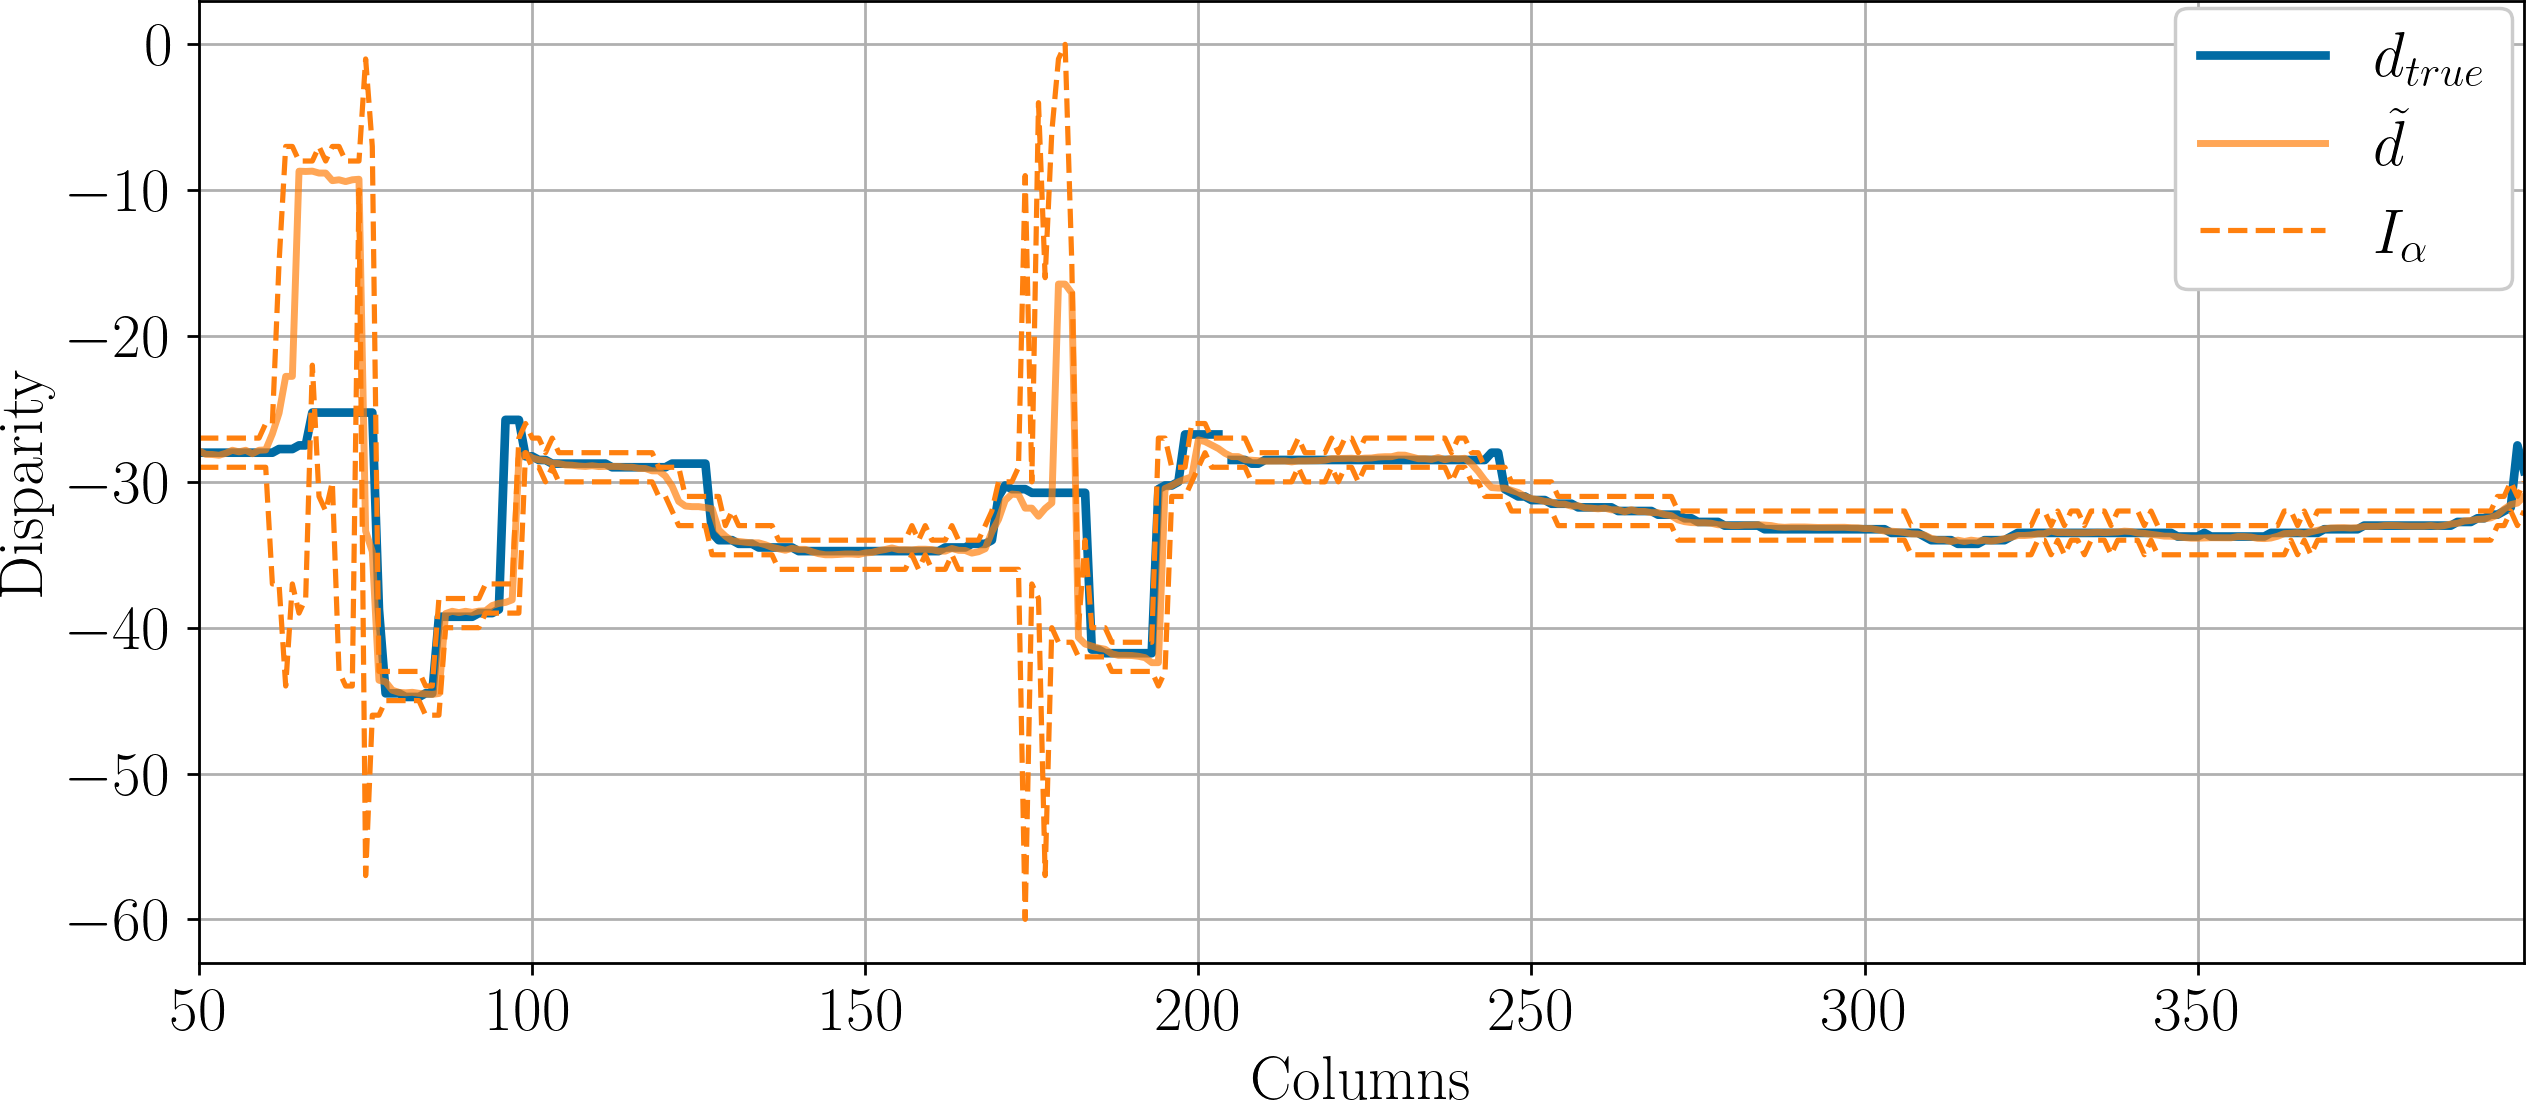
\includegraphics[width=\linewidth]{Images/Chap_5/intervals_ambiguous_area_row_180_1.png}
        \caption{$I_\alpha$ without regularization in low confidence areas}
        \label{fig:intervals_ambiguous_row_180_1}
    \end{subfigure}\hfill
    \begin{subfigure}[t]{\linewidth}
        \centering
        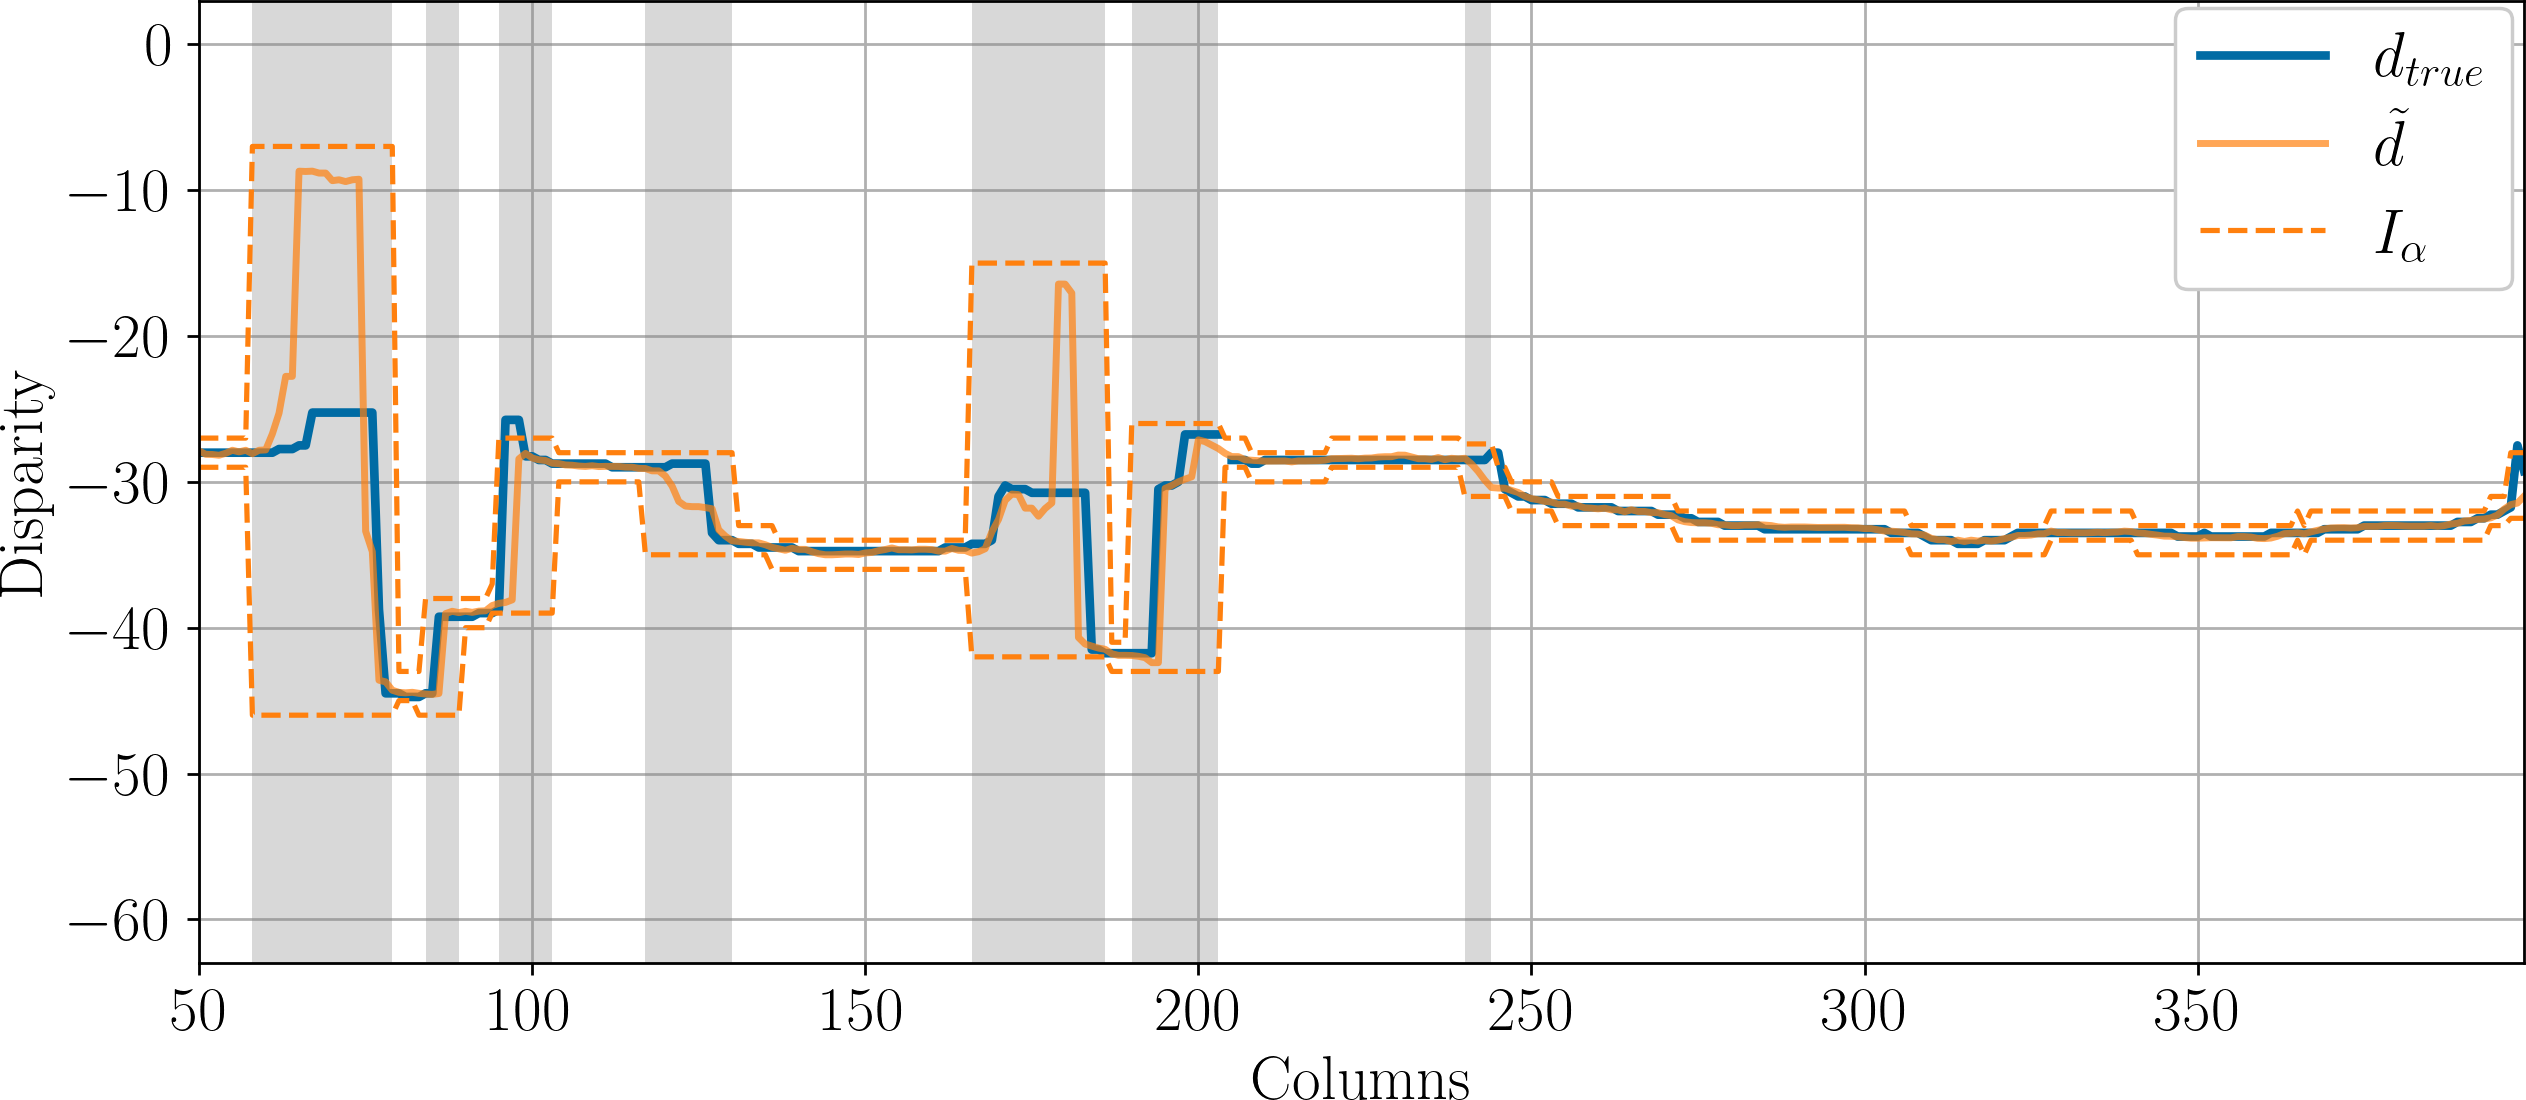
\includegraphics[width=\linewidth]{Images/Chap_5/intervals_ambiguous_area_row_180_2.png}
        \caption{$I_\alpha$ with regularization in low confidence areas}
        \label{fig:intervals_ambiguous_row_180_2}
    \end{subfigure}
    \caption{$I_\alpha$ with and without regularization in low confidence area, for row $180$ of the image of \Cref{fig:cones_with_rows}. Low confidence areas are indicated by the gray areas.}
    \label{fig:intervals_ambiguous_row_180}
\end{figure}

\begin{figure}
    \centering
    \begin{subfigure}[t]{\linewidth}
        \centering
        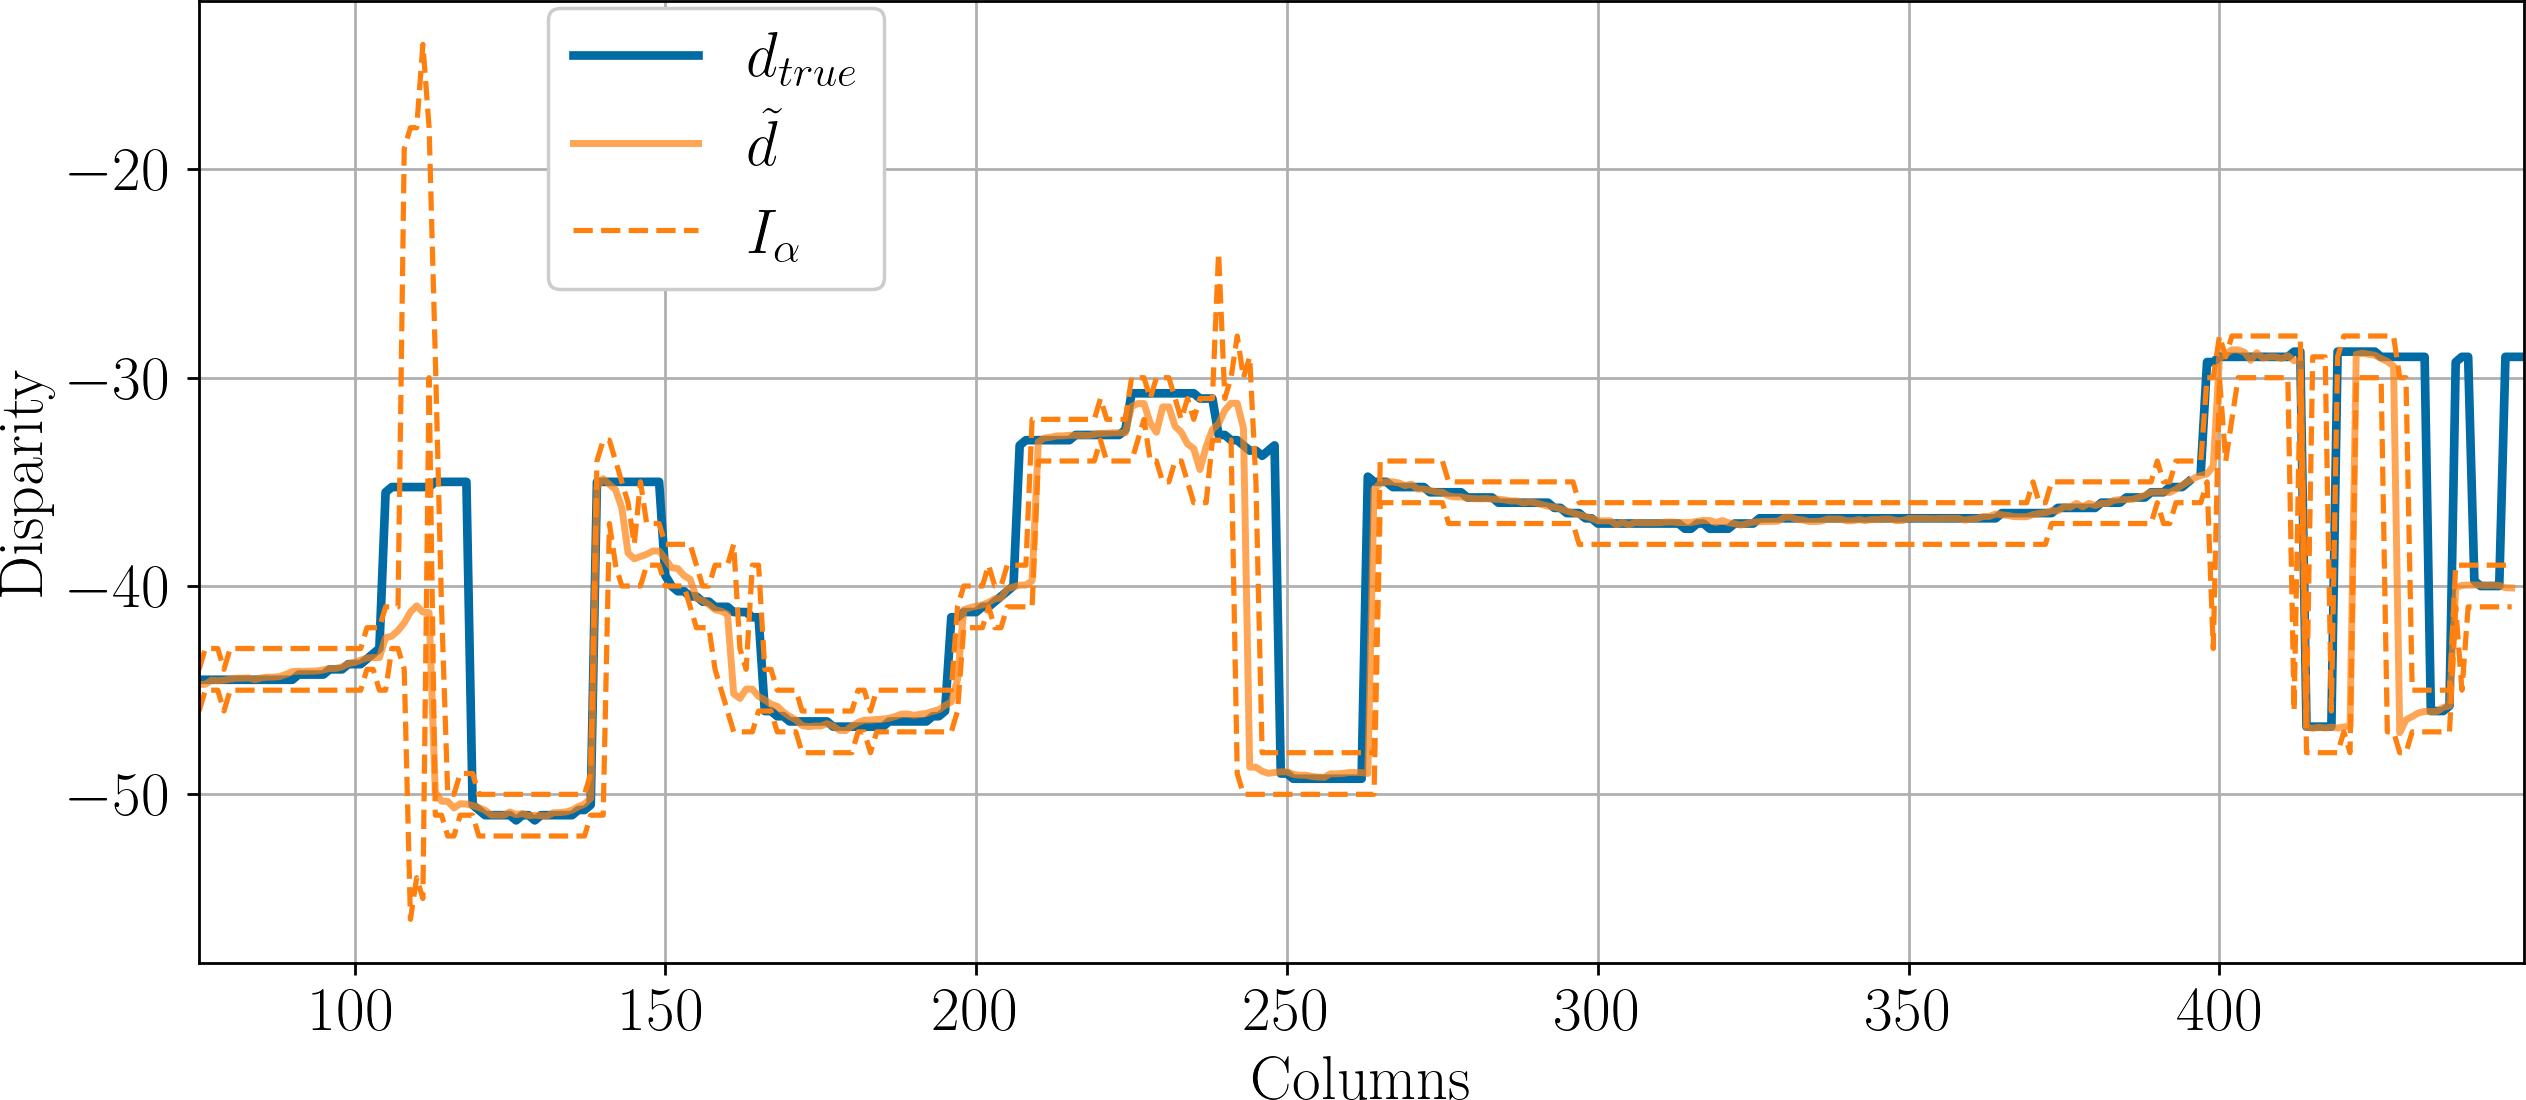
\includegraphics[width=\linewidth]{Images/Chap_5/intervals_ambiguous_area_row_240_1.png}
        \caption{$I_\alpha$ without regularization in low confidence areas}
        \label{fig:intervals_ambiguous_row_240_1}
    \end{subfigure}\hfill
    \begin{subfigure}[t]{\linewidth}
        \centering
        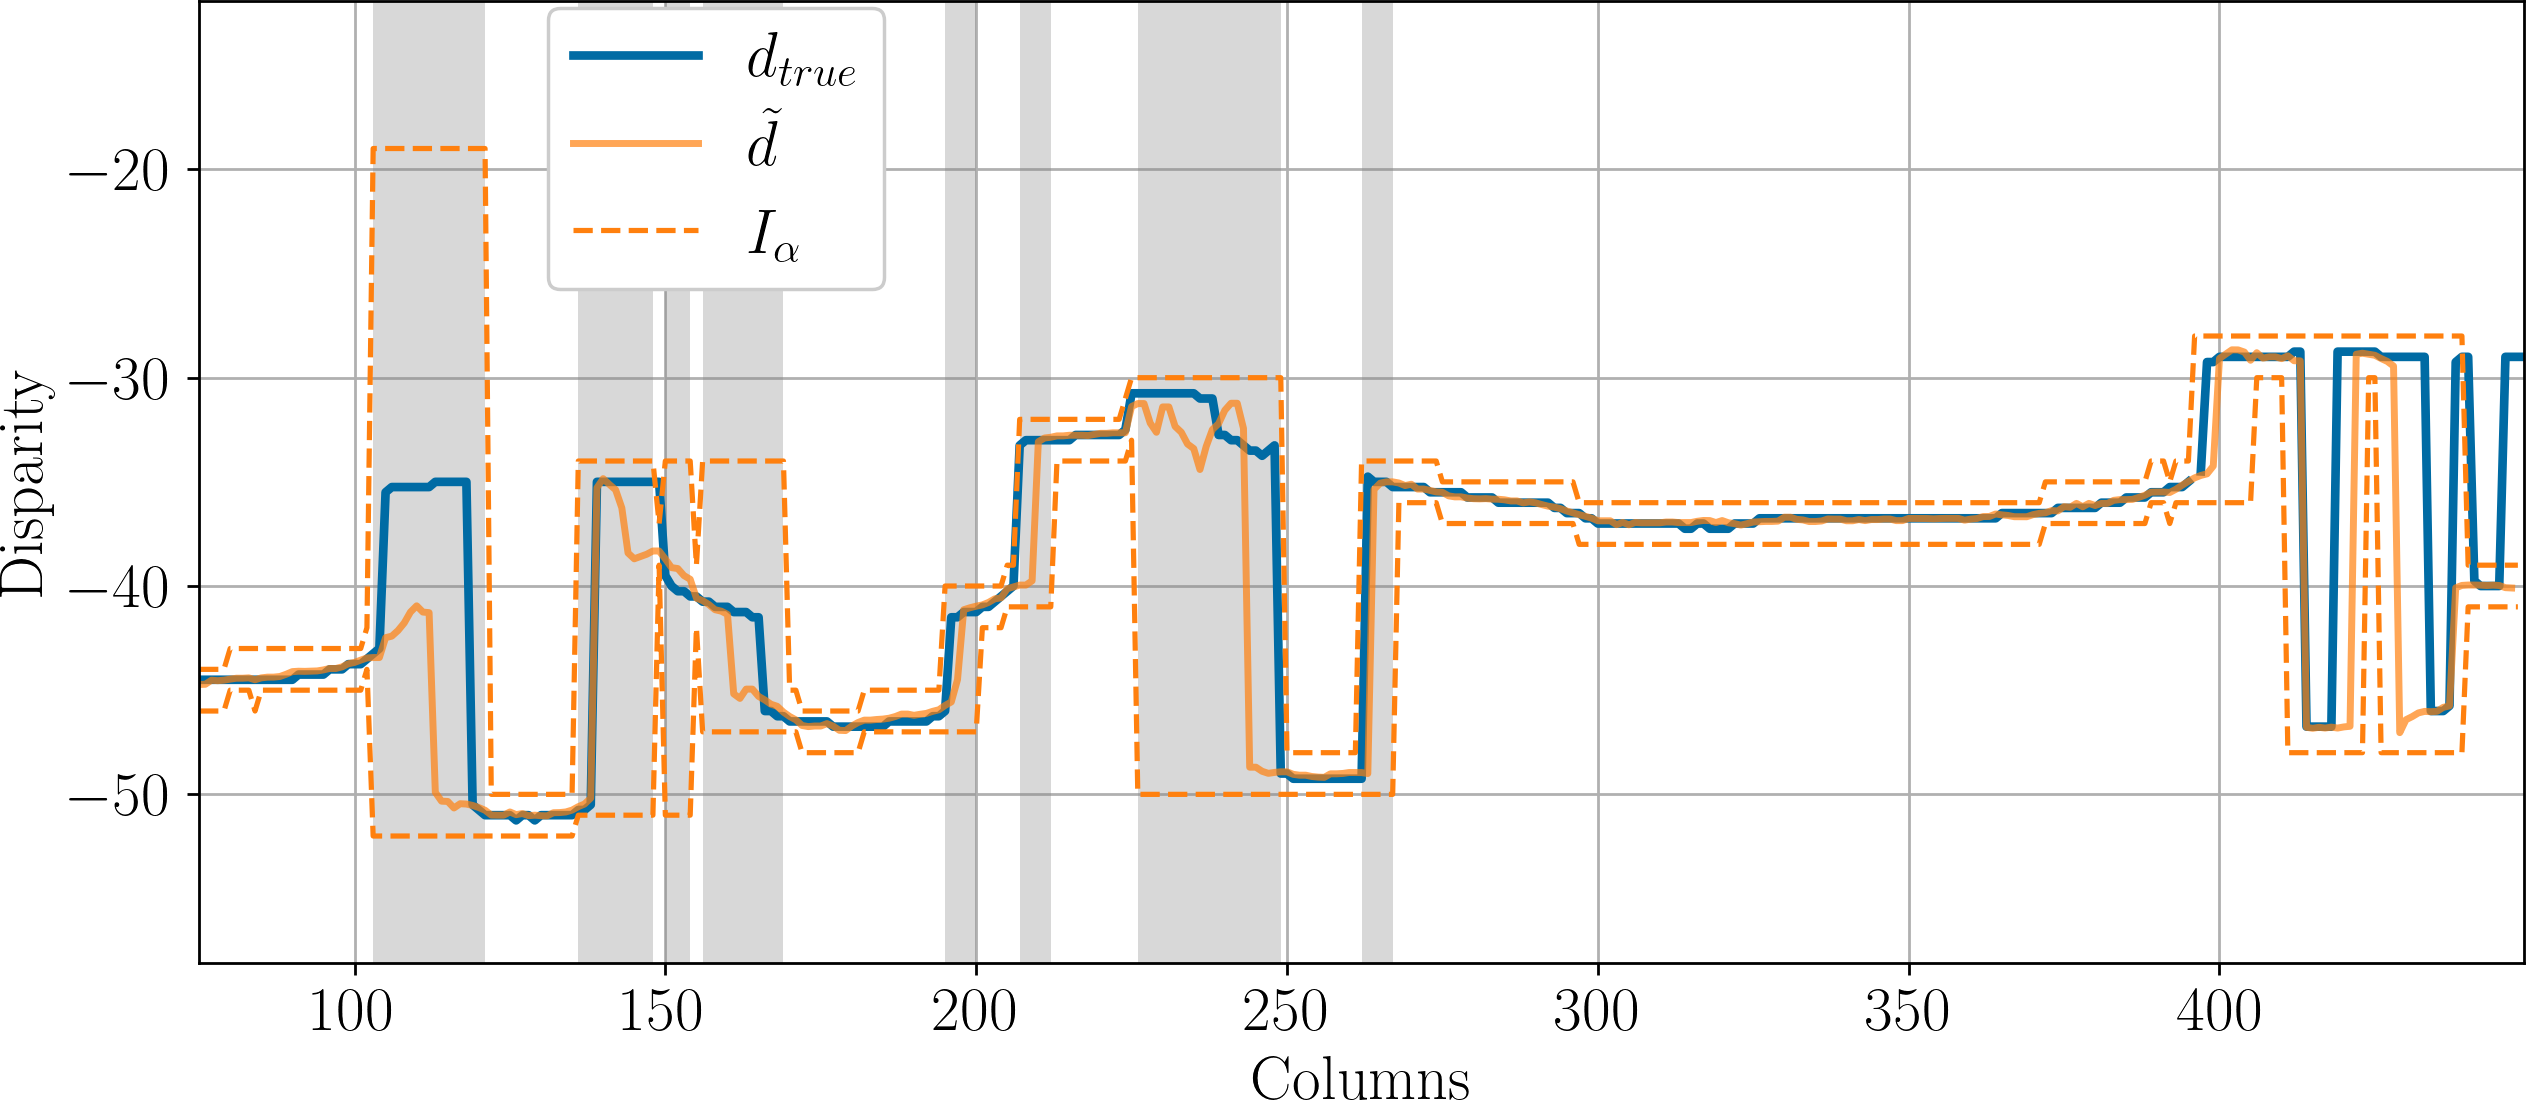
\includegraphics[width=\linewidth]{Images/Chap_5/intervals_ambiguous_area_row_240_2.png}
        \caption{$I_\alpha$ with regularization in low confidence areas}
        \label{fig:intervals_ambiguous_row_240_2}
    \end{subfigure}
    \caption{$I_\alpha$ with and without regularization in low confidence area, for row $240$ of the image of \Cref{fig:cones_with_rows}. Low confidence areas are indicated by the gray areas.}
    \label{fig:intervals_ambiguous_row_240}
\end{figure}

\begin{figure}
    \centering
    \begin{subfigure}[t]{\linewidth}
        \centering
        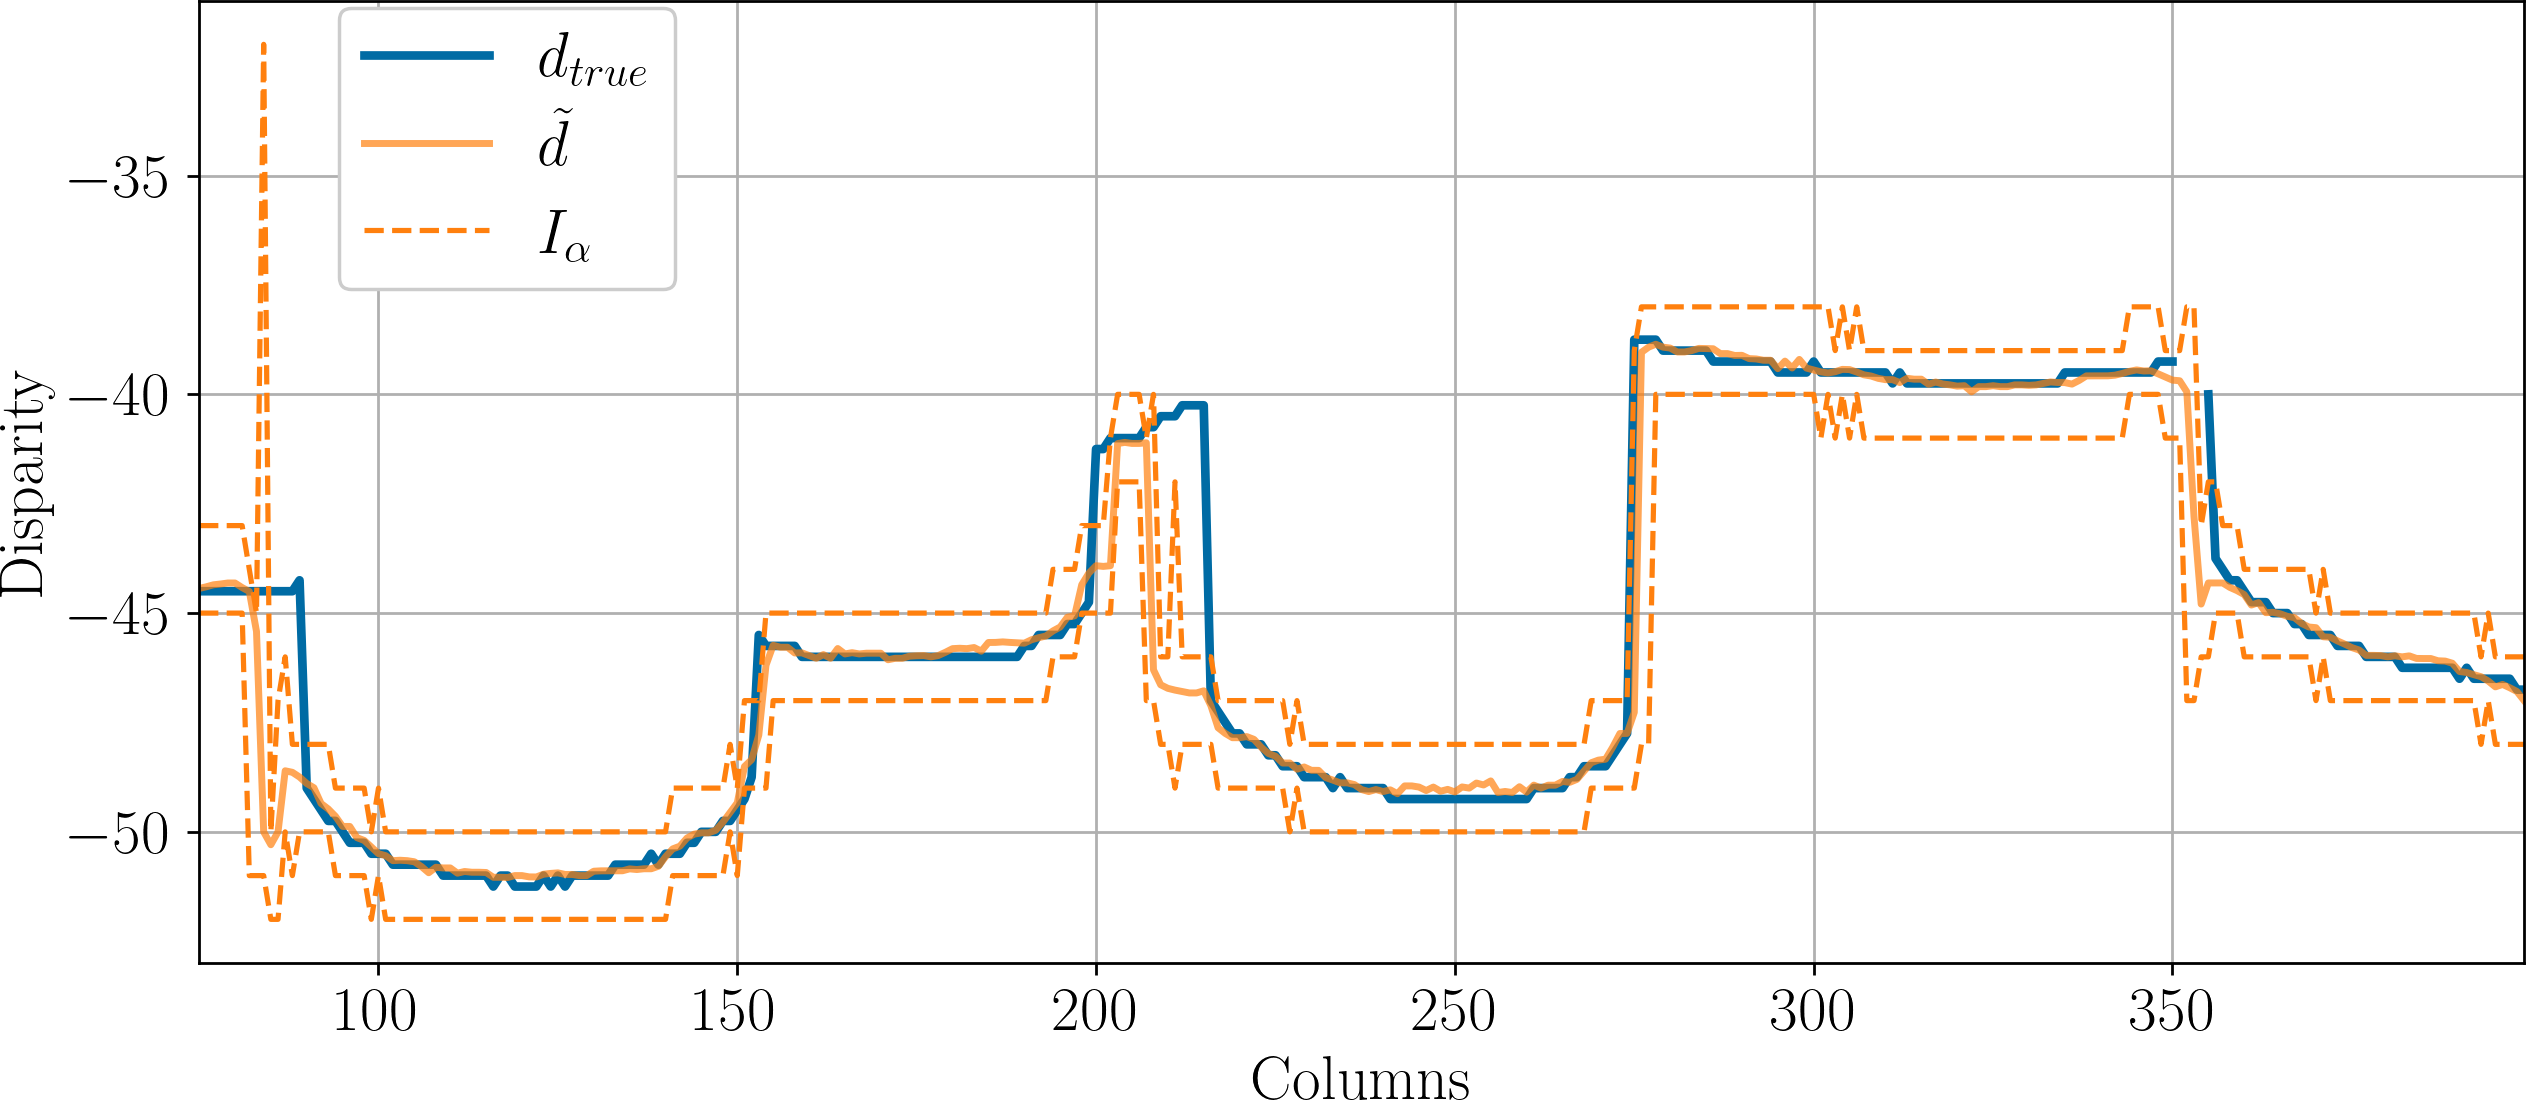
\includegraphics[width=\linewidth]{Images/Chap_5/intervals_ambiguous_area_row_290_1.png}
        \caption{$I_\alpha$ without regularization in low confidence areas}
        \label{fig:intervals_ambiguous_row_290_1}
    \end{subfigure}\hfill
    \begin{subfigure}[t]{\linewidth}
        \centering
        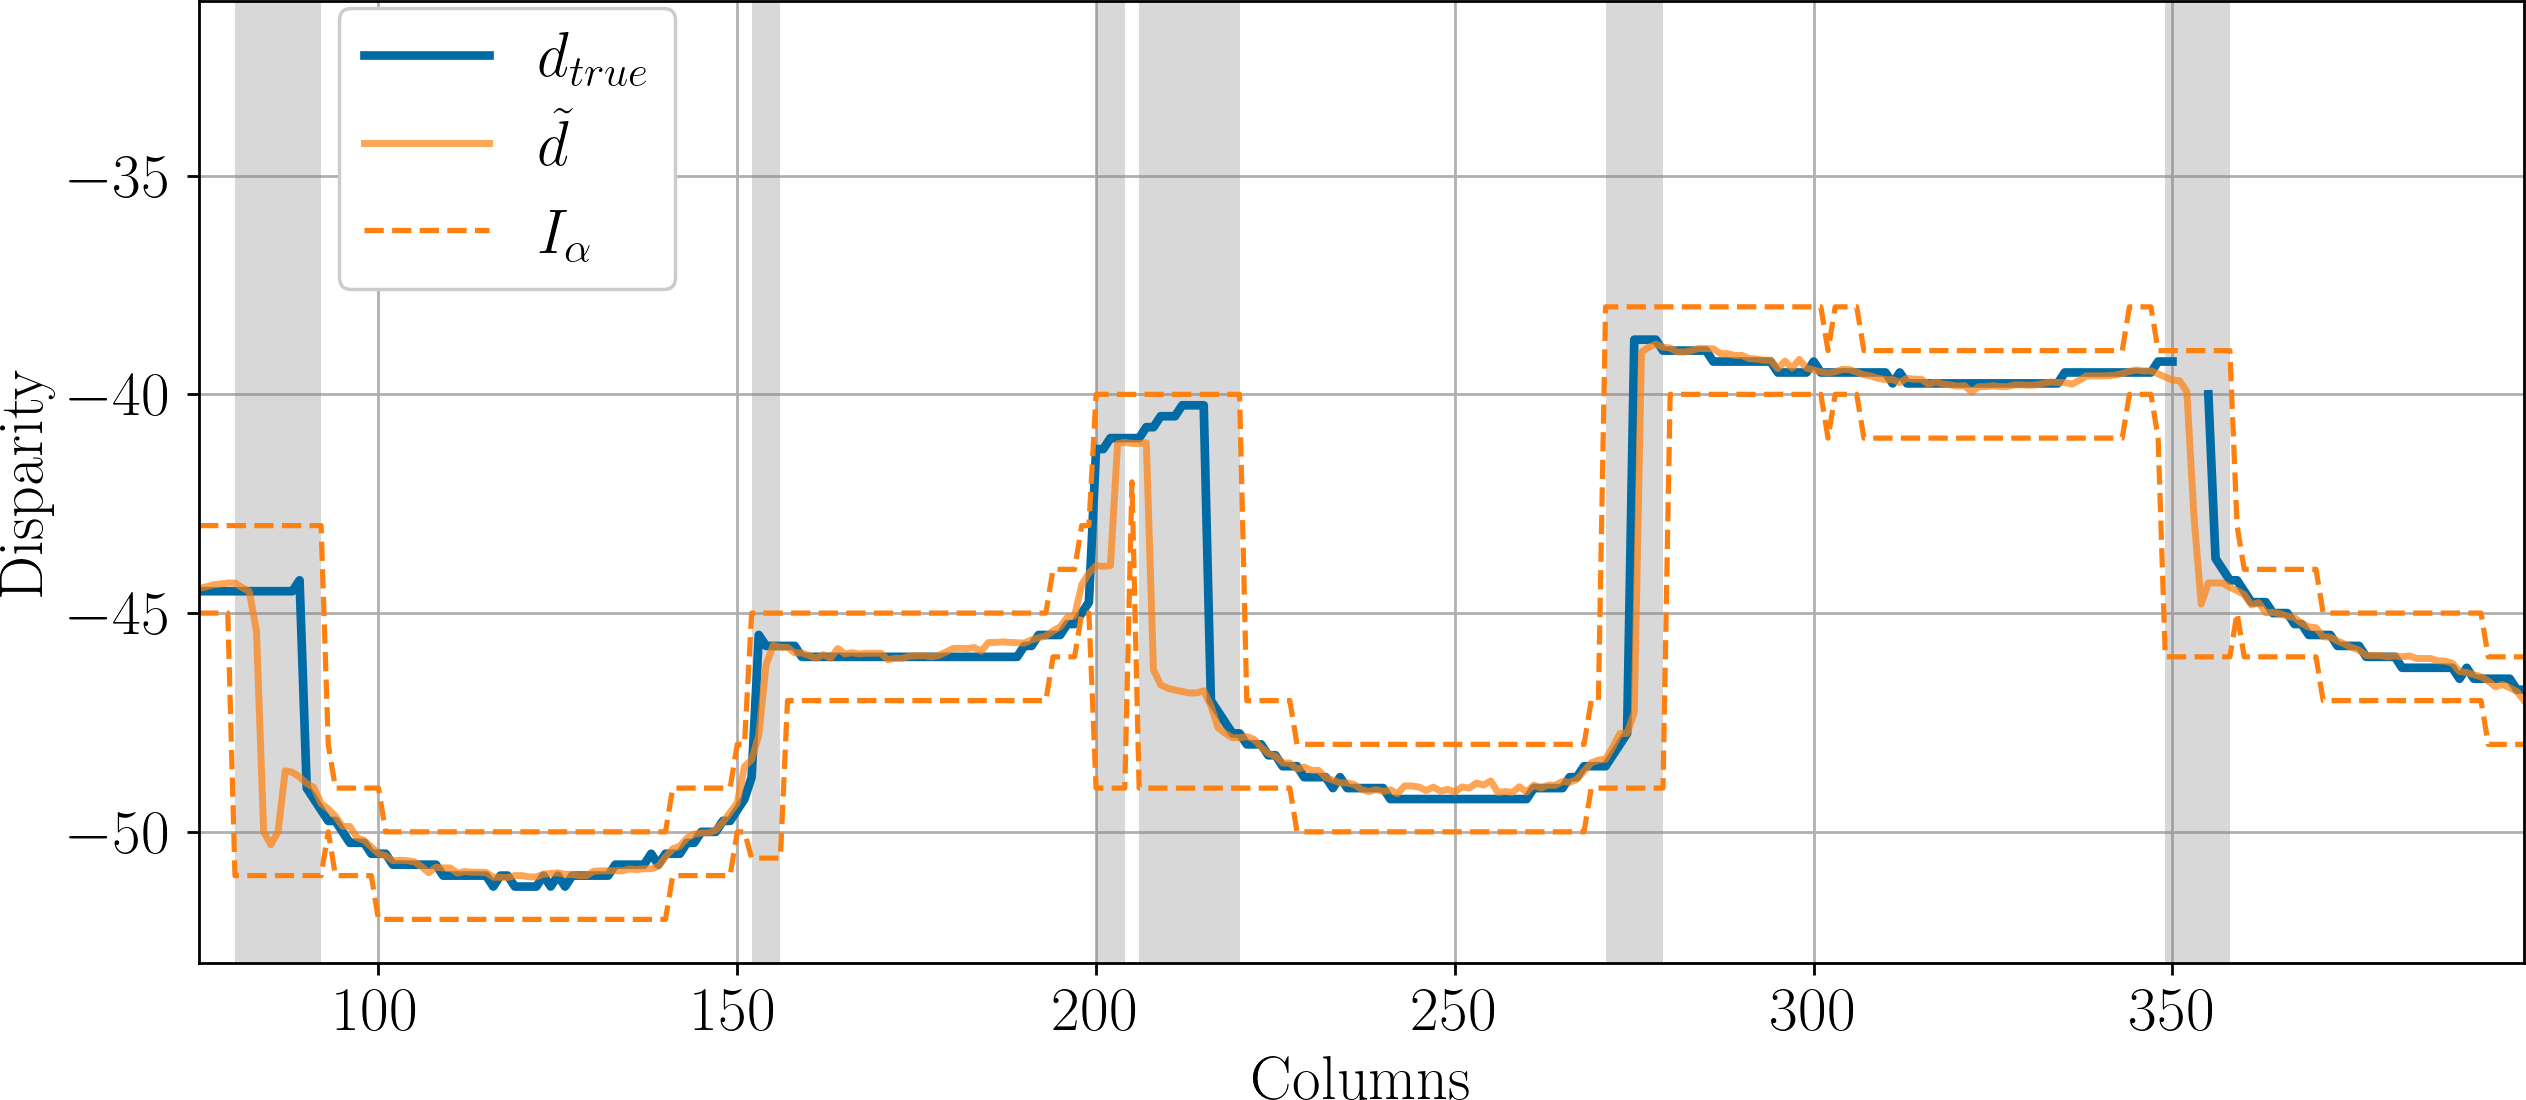
\includegraphics[width=\linewidth]{Images/Chap_5/intervals_ambiguous_area_row_290_2.png}
        \caption{$I_\alpha$ with regularization in low confidence areas}
        \label{fig:intervals_ambiguous_row_290_2}
    \end{subfigure}
    \caption{$I_\alpha$ with and without regularization in low confidence area, for row $290$ of the image of \Cref{fig:cones_with_rows}. Low confidence areas are indicated by the gray areas.}
    \label{fig:intervals_ambiguous_row_290}
\end{figure}

\todoroman{Attention Manue je m'en suis arrêté là :) }
Simple seuil mais avec une base théorique

\todoroman{Déplacer la phrase qui suit:} This model will however encounter some limitations in regions near depth discontinuities: as the \acrshort{sgm} regularization attempts to impose continuity on disparities, it results in cost curves that do not favor the correct disparity. Considering that the cost curves are equivalent to experts opinion in those areas can be over optimistic. We will see how we can adapt the model on those regions later in this section.

Ambiguity et régularization dans les zones de faibles confiance etc

\todoroman{Utilisation de l'ambiguité. Montrer differentes zones d'aggrégation avec différents paramètres. Dire qu'on pourrait utiliser toute bonne mesure de confiance, mais celle-ci à l'avantage d'être explicable, efficace, et déjà implémentée et utilisée dans la chaine CARS. Filtrage de la carte de disparité.}
\todoroman{Soit je mets les résultats des tests de disparité ici, soit je les mets après avoir fait tout le pipeline CARS.}
\todoroman{Expliquer aussi comment on peut remonter le LiDAR HD en géométrie Epi + rasterization.}

\subsection{Propagation in the CARS Pipeline}
Rasterization and small ideas with Gabriela?
Impact of tiling : cost volume min and max is not the same from one tile to another (statistically it should be close, provided that the tile is big enough and the disparity interval is also large enough)

\subsection{Unexplored leads}
Patatoides sur les lignes de visées. Un pixel est représenté par des coordonées précises mais est en fait l'aggrégation d'information radiométriques issues d'une surface au sol. On pourrait donc imaginer que les lignes de visées ne sont pas une ligne mais plus un cône/cylindre (approx), et donc qu'on pourrait donc représenter la position d'un point 3D comme l'intersection de deux volumes (cône + intervalles de disparité).   

\section{Coregistration}
DEM Compare 


\section{Evaluation of Disparity Intervals}
\section{Ablation Studies}
\section{Elevation Confidence Intervals}
\begin{table}[ht]
    \centering
    \begin{tabular}{|c||c|c|c|c|}
    \hline
        Area & Date for LiDAR & Date of Pléiades & Coupling mode & GT Size (0.5m)\\
        \hline\hline
        Bordeaux & 2023-09-15 & 2022-08-04 & Stereo & $6001\times 6001$\\\hline
        Grenoble & 2021-09-05 & 2020-09-17 & Stereo & $10 001\times 10 001$ \\\hline
        Jotunheinem & 2019-08-27 & 2019-08-27 & Stereo & \begin{tabular}{@{}c@{}} $7127\times 7298$ and\\ $3912\times2880$\end{tabular} \\\hline
        Langfjordjokelen & 2018-09-01 & 2018-09-01 & Stereo & $5841\times 3689$\\\hline
        Monaco & 2021-05-13 & 2020-08-30 & Stereo & $10 001\times 10 001$\\\hline
        Montpellier & 2021-05-28 & 2021-10-17 & Tri Stereo & $8001\times 8001$\\\hline
        Paris & 2023-03-03 & 2023-05-31 & Tri stereo & $10 001\times 10 001$\\\hline
        Peyto & 2016-09-13 & 2016-09-13 & Stereo & $13240\times 17874$\\\hline
        Pic du Midi & 2021-10-02 & 2021-10-16 & Stereo & $10001 \times 12001$ \\\hline
        Toulouse & 2022-05-29 & 2022-06-28 & Tri Stereo & $12001\times 8001$\\\hline
        Yosemite 1 &  \begin{tabular}{@{}c@{}} \tiny{2017-05-02 (snow) +} \\ \tiny{2014-08-27 (LiDAR)}\end{tabular} &  2017-05-01 & Tri stereo & \tiny{$17733\times 16800$ (3m)}\\\hline
        Yosemite 2 &  \begin{tabular}{@{}c@{}} \tiny{2017-05-02 (snow) +} \\ \tiny{2014-08-27 (LiDAR)}\end{tabular} &  2017-05-02 &  Tri stereo & \tiny{$17733\times 16800$ (3m)}\\ \hline
    \end{tabular}
    \caption{Acquisition date of Pléiade stereo or tri-stereo images, and the LiDAR ground truth}
    \label{tab:dates_pleiades_lidar_hd}
\end{table}

\begin{table}[ht]
    \centering
    \begin{tabular}{|c||c|c|c|c|}
    \hline
        Area & Date for LiDAR & Date of Pléiades & Coupling mode & GT Size (0.5m)\\
        \hline\hline
        Bordeaux & 2023-09-15 & 2022-08-04 & Stereo & $6001\times 6001$\\\hline
        Grenoble & 2021-09-05 & 2020-09-17 & Stereo & $10 001\times 10 001$ \\\hline
        Monaco & 2021-05-13 & 2020-08-30 & Stereo & $10 001\times 10 001$\\\hline
        Montpellier & 2021-05-28 & 2021-10-17 & Tri Stereo & $8001\times 8001$\\\hline
        Paris & 2023-03-03 & 2023-05-31 & Tri stereo & $10 001\times 10 001$\\\hline
        Pic du Midi & 2021-10-02 & 2021-10-16 & Stereo & $10001 \times 12001$ \\\hline
        Toulouse & 2022-05-29 & 2022-06-28 & Tri Stereo & $12001\times 8001$\\\hline
    \end{tabular}
    \caption{Acquisition date of Pléiade stereo or tri-stereo images, and the LiDAR ground truth}
    \label{tab:my_label}
\end{table}

\todoroman{Rasterizer le min max du lidar HD pour avoir une idée des intervalles.}
\pagebreak
\blankpage